\chapter{Jaynes-Cummings de dos átomos con medio y acoplamiento no lineal}
\label{ch4_dinamica}

%CAMBIAR ESTO PARA PERSONALIZARLO A MI GUSTO
\pagestyle{fancy}
\fancyhf{}
\fancyhead[LE]{\nouppercase{\rightmark\hfill}}
\fancyhead[RO]{\nouppercase{\leftmark\hfill}}
\fancyfoot[LE,RO]{\hfill\thepage\hfill}

En este capítulo se extiende el modelo de Jaynes-Cummings presentado en el capítulo \ref{ch3_jcm}. Lo más importante es que ahora se tienen dos átomos dentro de una misma cavidad. En la literatura en general, el modelo de JC fue extendido para considerar dos cavidades donde cada una tiene su propio átomo, y usando una condición inicial entrelazada se puede hacer interactuar ambas cavidades. El camino que se tomó en este trabajo, es un tanto fuera de lo convencional ya que no hay muchos estudios sobre este sistema. El principal obstáculo que presenta este problema, es que el espacio de Hilbert crece mucho y se torna inmanejable analíticamente. Como bien es sabido, el JCM tiene subespacios de 2 dimensiones que no se mezclan, y utilizando esta estrategia  se tendrán subespacios de 4x4 que tampoco se mezclan en el caso unitario. Esto permite encontrar algunas expresiones analíticas, pero en general se utilizaran métodos numéricos para analizar la dinámica. \newline
Este capítulo entonces seguirá un hilo conductor, partiendo desde el caso más sencillo hasta llegar a analizar cuales son los efectos de los diferentes parámetros en el problema, y particularmente se considerarán los efectos que estos tienen sobre la dinámica de entrelazamiento entre los dos átomos. 
Primero se resolverá el problema unitario de manera exacta, y se analizan las energías. Luego, para comprender las partes del problema, se aislará uno de los dos átomos, haciéndolo invisible a las interacciones con el otro átomo y con la cavidad. El objetivo de esto será recuperar numéricamente los resultados del capítulo anterior. Al terminar este análisis, se seguirá por recuperar las interacciones del átomo que se aisló del sistema teniendo el problema completo, y se estudiará la dinámica poblacional y principalmente la dinámica de entrelazamiento entre los dos átomos. El efecto que tienen las interacciones del problema sobre el entrelazamiento será la ultima parte del capítulo. Estudiar el entrelazamiento entre los dos átomos promete aplicaciones para estudiar la fidelidad de compuertas cuánticas.
%Primero se considera una cavidad perfecta, es decir sin disipaci\'on, agregándole el segundo átomo, vamos a intentar de entender cual es el efecto de este sobre el modelo de un solo átomo. Para esto haremos un análisis poblacional, y de observables como la entropía reducida, la concurrencia, las matrices de Pauli. Una vez agregado el segundo átomo, vamos a prender las interacciones de a una y vamos a analizar cuales son sus efectos. Luego, vamos a comparar esto con el caso en donde la cavidad presenta pérdidas. Principalmente, nos centraremos en un análisis del entrelazamiento, ya que esta es la cualidad más interesante que tenemos en el ámbito de la informaci\'on cu\'antica. 



\section{Modelo de dos átomos y solución unitaria}
Este trabajose concentra en una extensión del modelo, donde se ubican dos átomos dentro de la cavidad. Estos átomos pueden interactuar entre si, y con la cavidad, y además se consideran no-linealidades en el acoplamiento y en el medio.
Se utiliza un modelo de Jaynes-Cummings para describir la interacci\'on entre el campo electromagn\'etico y los átomos. Adem\'as se supondrá que el acoplamiento depende de la cantidad de fotones y los átomos podr\'an interactuar entre sí mediante un término tipo Ising y otro tipo dipolo-dipolo. Recordemos que se asume que vale la aproximaci\'on de onda rotante ($\omega_0 \sim \omega$) y $g << \omega,\omega_0$.
Entonces, el Hamiltoniano que describe este problema es el siguiente ($\hbar=1$):
\begin{equation}
\begin{split}
     \hat H & =\underbrace{ \omega_0 h(\hat n) \hat n }_{\hat H_F}+\underbrace{\frac{ \omega}{2}(\hat\sigma_Z^{(1)}+\hat\sigma_Z^{(2)})}_{\hat H_A}   \\ 
     & + \underbrace{ g(\hat\sigma_+^{(1)}\hat a f(\hat n)+\hat\sigma_-^{(1)}f(\hat n) \hat a^\dagger + \hat\sigma_+^{(2)}\hat a f(\hat n)+\hat\sigma_-^{(2)}f(\hat n) \hat a^\dagger)}_{H_{FA}} \\ +& \underbrace{2 \kappa (\hat \sigma_-^{(1)}\hat \sigma_+^{(2)}+\hat \sigma_+^{(1)}\hat \sigma_-^{(2)}) +  J \hat \sigma_Z^{(1)}\hat \sigma_Z^{(2)}}_{H_{AA}},
\end{split}
\end{equation}
donde $\hat a$ es el operador de aniquilaci\'on del fot\'on, $\omega_0$ y $\omega$ son las frecuencias del fot\'on y del átomo respectivamente, $g$ es la constante de acoplamiento, las constantes $J$ y $\kappa$ son los par\'ametros de Ising y de dipolo-dipolo para las interacciones átomo-átomo, y los operadores $\hat \sigma^{(i)}$ son las matrices de Pauli que act\'uan sobre el átomo i-esimo. Finalmente, las funciones $h(\hat n)$ y $f(\hat n)$ son las que van a dar cuenta de la no linealidad dependiente del número de fotones de la cavidad $\hat n = \hat a^\dagger \hat a$. 

Un medio tipo Kerr está descrito por la funci\'on $h(\hat n)=1+\frac{\chi}{\omega_0}\hat n$ \cite{Lugiato1987}, y la funci\'on $f(\hat n)$ describe el tipo de acoplamiento, de las cuales se consideran dos opciones: si el acoplamiento es lineal $f(\hat n)=1$, y si el acoplamiento es no lineal, especificamente se considera de tipo Buck-Sukumar $f(\hat n) = \sqrt{\hat n}$ \cite{Buck1980}.

En este punto es útil hacer una transformaci\'on unitaria  $K = \exp\left\{-i \omega t (\hat a^\dagger \hat a + \hat \sigma_z/2)\right\}$ para dejar el Hamiltoniano en funci\'on del Detuning $\Delta (\sim 0)$. 

\begin{equation}
\begin{split}
     \hat H_I & = \chi \hat n^2+\frac{ \Delta}{2}(\hat\sigma_Z^{(1)}+\hat\sigma_Z^{(2)})   \\ 
     & +  g(\hat\sigma_+^{(1)}\hat a f(\hat n)+\hat\sigma_-^{(1)}f(\hat n) \hat a^\dagger + \hat\sigma_+^{(2)}\hat a f(\hat n)+\hat\sigma_-^{(2)}f(\hat n) \hat a^\dagger) \\ 
 & + 2 \kappa (\hat \sigma_-^{(1)}\hat \sigma_+^{(2)}+\hat \sigma_+^{(1)}\hat \sigma_-^{(2)}) +  J \hat \sigma_Z^{(1)}\hat \sigma_Z^{(2)}
\end{split}
\end{equation}\label{ec4:H}
Este es el Hamiltoniano con el que se trabaja, así que a partir de ahora el subíndice I es redundante y se dejará implícito. Obsérvese que el caso de $\chi=0$ es el caso de un medio lineal. 


Este Hamiltoniano se puede resolver analíticamente para el caso de una cavidad sin pérdidas \cite{Santos2016}. Para resolver el problema lo primero que se nota es que el Hamiltoniano conserva el número de excitaciones, es decir $[H,\hat N]=0$, y en esta situación es sabido que el Hamiltoniano de JC es diagonal por bloques si se elige convenientemente la base. Esta es la que agrupa los estados con misma cantidad de excitaciones $\hat N = \hat n + \hat \sigma_+^{(1)}\hat \sigma_-^{(1)}+\hat \sigma_+^{(2)}\hat \sigma_-^{(2)}$: 
\begin{equation}
\begin{split}
    \mathcal{B}_n=& \left\{\ket{\Phi^{(n)}_1}=\ket{ggn},\ket{\Phi^{(n)}_2}=\frac{1}{\sqrt{2}}(\ket{egn-1}+\ket{gen-1}),\ket{\Phi^{(n)}_3}=\ket{een-2},\right. \\
& \left. \ket{\Phi^{(n)}_4}=\frac{1}{\sqrt{2}}(\ket{egn-1}-\ket{gen-1})\right\} ,
\end{split}
\label{ec4:base}
\end{equation}
donde se eligi\'o esta combinaci\'on particular porque el último estado de la base, que es impar ante intercambio, queda desacoplado de los otros, simplificando el problema. Esto se ve al evaluar los elementos de matriz del Hamiltoniano $H_{i,j}=\bra{\Phi_i}\hat H \ket{\Phi_j}$. El subespacio correspondiente a $n$ excitaciones $\hat H^{(n)}$ es una matriz de 4x4
\begin{equation}
    \hat H^{(n)}=
    \begin{pmatrix}
     \chi n^2 - \Delta +  J & \sqrt{2} g f(n)\sqrt{n} & 0 & 0 \\
    \sqrt{2} g f(n)\sqrt{n} &  \chi (n-1)^2  -  J + 2 k & \sqrt{2} g f(n-1)\sqrt{n-1} & 0 \\
    0 & \sqrt{2} g f(n-1)\sqrt{n-1} &  \chi (n-2)^2 +  \Delta +  J & 0 \\
    0&0&0& \begin{aligned} 
                 & \chi (n-1)^2  \\ 
                 &-  J - 2 k
        \end{aligned}
    \end{pmatrix}
\end{equation}
Se ve claramente que el estado impar ante intercambio está aislado, y entonces es autoestado del problema, y por lo tanto evoluciona solo y no se mezcla con los otros estados. Esto nos sirve porque ahora, para terminar de resolver el problema, tenemos que diagonalizar la matriz de 3x3. Cabe aclarar que esta matriz solo es válida para $n\geq 2$, ya que los subespacios con $N=0,1$ no tienen 4 estados. En estos casos la soluci\'on del problema de autovalores es más sencilla aún, as\'i que solo se muestran los resultados. \newline
Para resolver el problema de autovalores de la matriz de 3x3 se utiliza la fórmula de Cardano para conseguir las ra\'ices triples que aparecen en el polinomio caracter\'istico, cuyos autovalores son
\begin{equation}
    E_j^{(n)}=-\frac{1}{3}\beta_n+2\sqrt{-Q_n}\cos{\left(\frac{\theta_n+2(j-1)\pi}{3}\right)},
    \label{ec4:autoenergias}
\end{equation}
para $j=1,2,3$, y donde:
\begin{equation}
    \theta_n=\cos^{-1}\left(\frac{R_n}{\sqrt{-Q_n^3}}\right),
\end{equation}
\begin{equation}
    \begin{aligned}
        Q_n & = \frac{3\gamma_n-\beta_n^2}{9} ,\\
        R_n & = \frac{9\beta_n\gamma_n-27\eta_n-2\beta_n^3}{54} ,\\
        \beta_n & = - \left( \chi(n^2+(n-1)^2+(n-2)^2)+J+2k\right) ,\\
        \gamma_n & = (\chi(n-1)^2 - J + 2k)(x(n-2)^2+\chi n^2+2J) \\ 
        & +(\chi (n-2)^2+\Delta+J)(x n^2-\Delta+J)-2g^2(n^{2a}+(n-1)^{2a}) ,\\ 
        \eta_n &= -(\chi n^2-\Delta+J)(\chi(n-2)^2+\Delta+J)(\chi(n-1)^2-J+2k) \\
        &+2g^2 \left[  \chi(n-2)^2n^{2a}+\chi n^2(n-1)^{2a}+\Delta\left(n^{2a}-(n-1)^{2a}\right) +J(n^{2a}+(n-1)^{2a})\right].
    \end{aligned} 
    \label{ec4:parametros solucion}
\end{equation}
donde $a=\frac{1}{2}$ se corresponde con acoplamiento lineal, es decir, $f(n)=1$, y $a=1$ a Buck-Sukumar $f(n)=\sqrt{n}$. Los autovalores ser\'an reales si $Q_n^3+R_n^2<0$.
Con esto podemos escribir los autovectores:
\begin{equation}
    \begin{split}
        \ket{u_j^{(n)}} &= \frac{1}{N_j^{(n)}} \bigg[ \left((E_j^{(n)} - H_{22}^{(n)})(E_j^{(n)}-H_{33}^{(n)}) - H_{23}^{(n)^2} \right) \ket{\Phi_1^{(n)}} \\ &+ H_{21}^{(n)}(E_j^{(n)}-H_{33}^{(n)})\ket{\Phi_2^{(n)}} + H_{23}^{(n)}H_{12}^{(n)}\ket{\Phi_3^{(n)}}\bigg].
    \end{split}
\end{equation}
Obviamente el último es el estado $\ket{\Phi_4^{(n)}}$, que también es autoestado, con autovalor $E_4^{(n)}=\chi(n-1)^2-J-2k$.
Para el subespacio de $N=0$ solo hay un vector $\ket{\Phi_1^{(0)}}=\ket{gg0}$ y su autovalor es $E_1^{(0)}=-\Delta+J$.
Para $N=1$ se tienen tres vectores en el subespacio, y las autoenergías son
\begin{align}\label{ec4:energias n1}
    E_{1,2}^{(1)} &=\frac{\chi -\Delta}{2} +k \pm \sqrt{2g^2+(k-J+\frac{\Delta -\chi}{2} )^2},\\
    E_3^{(1)} & = -2k-J,  
\end{align}
y sus autovectores
\begin{equation}
    \begin{aligned}
        \ket{u_{1,2}^{(1)}}&=\frac{1}{N_{1,2}^{(1)}}(-\sqrt{2}g\ket{gg1}+ \left(\frac{\chi-\Delta}{2}+J-k \mp \sqrt{2g^2+(k-J+\frac{\Delta -\chi}{2} )^2} \right)\dfrac{\ket{eg0}+\ket{ge0}}{\sqrt{2}},\\
        \ket{u_3^{(1)}}&= \frac{1}{\sqrt{2}}(\ket{eg0}-\ket{ge0}).
    \end{aligned}
\end{equation}

Con esto, se resuelve analíticamente la evolución temporal de cualquier estado inicial.
Para esto sólo es necesario desarrollar el estado inicial en términos de los autovectores, y la evolución temporal está dada por
\begin{equation}
\ket{\psi(t)}=e^{-iHt}\ket{\psi(0)}=\sum_{j,n} c_j^{(n)}e^{-iE_j^{(n)}t}\ket{u_j^{(n)}},
\end{equation}
donde $c_j^{(n)}=\braket{u_j^{(n)}}{\psi(0)}$.
La complejidad de estas expresiones hace complicado conseguir conclusiones interesantes, aún así, algo que se puede notar, es la diferencia fundamental entre las energías con un número total de excitaciones $N=1$ y $N>1$. El factor que está antes de la raíz cuadrada, para el caso en que $N \geq 2$ hay un $\frac{1}{3}\beta_n$ que solo depende de $\chi$, $J$, $k$ y $n$. Mientras que en el caso de $N=1$, este factor depende del detunning $\Delta$. Esto es interesante, ya que uno podría pensar que la formula para $N$ excitaciones se puede generalizar para incluir $N=0,1$, pero la diferencia fundamental de tener más o menos estados que interactúan entre si, da lugar a efectos fundamentalmente diferentes. Si se mira en detalle las cuentas, en el caso de $N=1$ este factor $\Delta$ aparece, ya que en la matriz Hamiltoniana el único estado con $N=1$ que tiene un término que incluye al detunning, es el estado $\ket{gg1}$. Por lo tanto, este término con $\Delta$ sobrevive, al contrario que en todos los demás subespacios, ya que por un lado el termino del $\ket{ggn}$ que aporta un $\Delta$, y el término de $\ket{ee,n-2}$ aporta otro $\Delta$ pero con el signo cambiado, y elimina la contribución del primer estado a la energía. La consecuencia de esto es que para $N=1$, si se aumenta el detunning, no solo se separan los niveles de energía, sino que también hay una asimetría por el término independiente. Para analizar esto en detalle, en la figura \ref{fig:relación energia detunning} se observan las energías de los diferentes niveles en función del detunning. 

\begin{figure}
    \centering
    \begin{subfigure}[h]{0.49\textwidth}
        \centering
        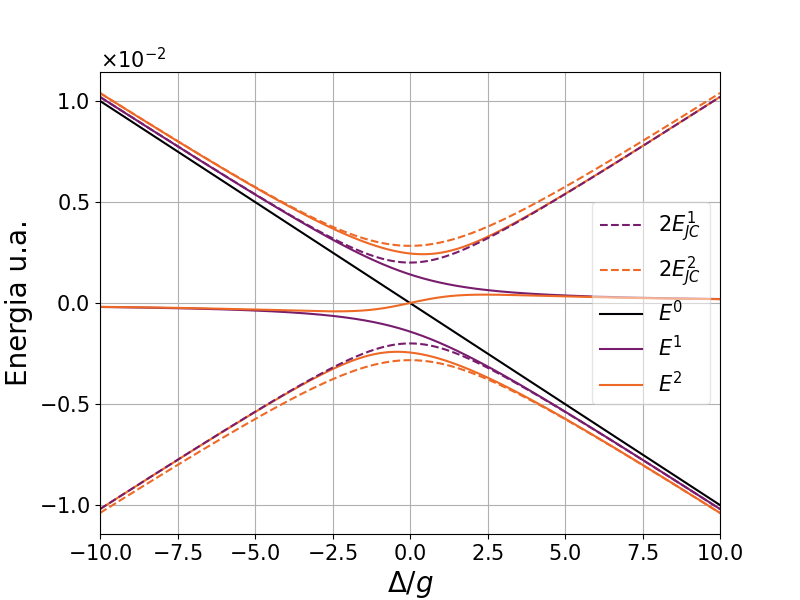
\includegraphics[width=\textwidth]{figuras/ch4/energias 0.png}
        \caption{}
        \label{fig:relación energia detunning 1}
    \end{subfigure}
    \hfill
    \begin{subfigure}[h]{0.49\textwidth}
        \centering
        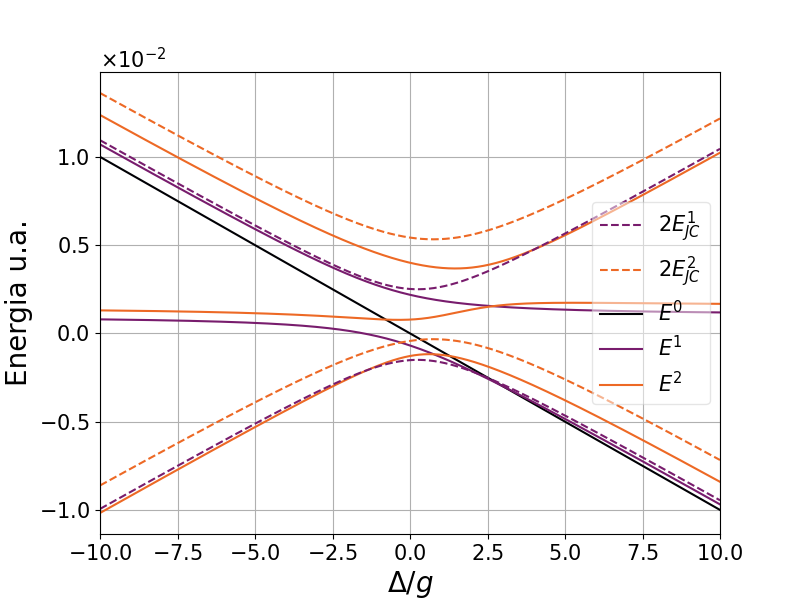
\includegraphics[width=\textwidth]{figuras/ch4/energias 0.5.png}
        \caption{}
        \label{fig:relación energia detunning 2}
    \end{subfigure}
       \caption{Relación entre energía y detunning para los diferentes niveles de energía del problema. Las líneas sólidas muestran la energía de los estados del JC doble con $N=0$ (negro, sólido), $N=1$ (violeta sólido) y $N=2$ (naranja sólido). También se muestran los niveles de energía del JC de un átomo para $N=1$ (negro; rayado) y $N=2$ (naranja; rayado). Obsérvese que las energías del JC de un átomo están multiplicadas por 2. (a) $\chi=k-J=0$; (b) $\chi=k-J=0.5g$}
       \label{fig:relación energia detunning}
\end{figure}
En la figura \ref{fig:relación energia detunning 1} se observan las energías de los primeros niveles para el modelo de un átomo (líneas rayadas), y de dos átomos (líneas sólidas); para esta figura se tomaron átomos que no interactúan ($k=J=0$) y una cavidad lineal ($\chi=0$). Se puede ver que, si bien el modelo de dos átomos tiene estructuras más complicadas, son similares a las de 1 átomo. En primer lugar, los estados con $N=2$ (naranja; sólido) tienen una forma igual a la de JC de 1 átomo, si bien está un poco desfasada, es interesante ver como las líneas tienen una coincidencia muy grande, recordando que en el gráfico las líneas rayadas están multiplicadas por 2, esto tiene una interpretación bastante buena, y es que la energía de dos átomos no interactuantes en una cavidad es igual (o muy parecida) a dos veces la energía de 1 átomo en una cavidad. Esta diferencia se debe al corrimiento Lamb, ya que ahora tenemos dos átomos que interactúan con el vacío, este tiene una forma un poco diferente:
\begin{equation}
    \begin{aligned}
        \Delta E_{1}&=E^{n}_1-E^{(0)}_1=\frac{g^2}{\Delta}(2n-1) \\
        \Delta E_{2}&=E^{n}_1-E^{(0)}_1=-\frac{g^2}{\Delta}(2n-1) \\
        \Delta E_3 &=0
    \end{aligned}
\end{equation}
Las tres autoenergías presentan correcciones del orden de $\frac{g^2}{\Delta}$ en su valor asintótico, pero la dependencia cambia con respecto al caso de 1 átomo, lo que explica las diferencias de la Figura \ref{fig:relación energia detunning 1}. Esta dependencia es sorprendente ya que no es simplemente el doble que el caso de 1 átomo. En la Figura \ref{fig:relación energia detunning 2}, donde hay interacción entre átomos, se pierde la analogía con el caso de 1 átomo.

Por otro lado, la energ\'ia de los estados con $N=1$ tienen un t\'ermino fuera de la raíz, que hace que sea más asim\'etrico a\'un. Normalmente, en el JC de 1 átomo, ya que todos los niveles de energía tienen la misma forma funcional, este término de afuera de la raíz se le puede agregar o quitar como un offset en la energía del estado fundamental, la diferencia con este caso es que, no todos los niveles de energía presentan esto, entonces si se agrega un offset, igualmente habría una diferencia. 

Una observación menor es que si la cavidad es lineal, entonces los estados antisimétricos de diferentes excitaciones $\frac{1}{\sqrt{2}}(\ket{eg,n}-\ket{ge,n})$ y $\frac{1}{\sqrt{2}}(\ket{eg,n'}-\ket{ge,n'})$, están degenerados en energía. Esto solo tiene importancia al considerar una cavidad con pérdidas.

Una vez estudiados los niveles de energía y comparados con el caso de 1 átomo, se prosigue con la dinámica del problema, que en el caso unitario puede resolverse analíticamente, pero a\'un así, la herramienta principal de análisis son las simulaciones numéricas.
Para comenzar se quiere recuperar el caso de un átomo. Para esto se trabaja con $k=J=0$ y se agrega un parámetro adimensional $\alpha$ que solamente actúa sobre el átomo B, y sirve de apantallamiento. Este parámetro $\alpha$ acompañará a las constantes de acoplamiento $g\rightarrow g\alpha$, tal que si $\alpha \rightarrow 0$ entonces el átomo se desacopla de la cavidad. 

\section{Dinámica con apantallamiento}
\label{sec4:dinamica apantallamiento}
Lo primero que se tiene que hacer es recuperar los resultados anteriores. Para aclarar, en la Figura \ref{fig4:diagrama esquematico} se muestra un esquema de como es el problema que se está trabajando, con los nombres que se le darán a las partes del sistema. Llamaremos átomo B al que está apantallado mediante el parámetro adimensional $\alpha$, el indice A se referirá al otro átomo, y C a la cavidad. Entonces, para recuperar los resultados anteriores, se propone que $\alpha=0$ y la interacción entre los átomos $k=J=0$. De esta manera, se elige en analogía con el caso de 1 átomo, como estado inicial cualquier estado donde el átomo A sea excitado, y la cavidad C no tenga ningún fotón; por lo tanto se elige el estado inicial más sencillo posible que cumple estas condiciones $\ket{\psi_0}=\ket{eg0}$. Si bien este apantallamiento no tiene un significado físico, y experimentalmente es imposible lograr estas condiciones, realizar este estudio sirve para entender cualitativamente los efectos de cada parámetro del problema, y también entender que el entrelazamiento entre los dos átomos, lleva a efectos impredecibles. La complejización del problema de 1 átomo al de 2 átomos es muy grande, y por eso es necesario ir de a poco.
\begin{figure}[h]
    \centering
    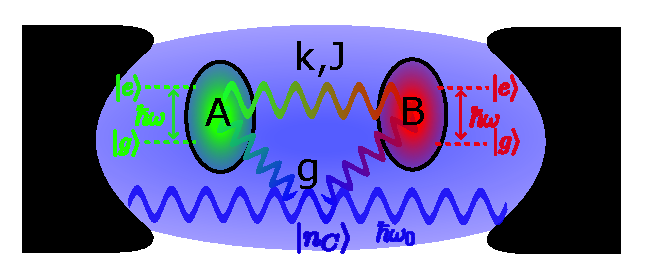
\includegraphics[width=\textwidth]{figuras/ch4/esquema.pdf}
    \caption{Esquema del problema de estudio. Se nombran a las partes para referenciarlas fácilmente: los átomos se identifican por las letras A y B, y la cavidad por la C, esta puede contener una cantidad arbitraria de excitaciones, pero se trabajará principalmente en 0,1 y 2 excitaciones. Ambos átomos son de dos niveles, son idénticos e indistinguibles y su frecuencia natural es $\omega$, mientras que la frecuencia natural de la cavidad es $\omega_0$. El acoplamiento entre la cavidad y el átomo es $g$, y las interacciones átomo-átomo son $k$ (interacción dipolar) y $J$ (interacción tipo Ising).}
    \label{fig4:diagrama esquematico}
\end{figure}
Utilizando esta condición inicial se realiza una simulación numérica y se observan las poblaciones, y se espera recuperar la misma dinámica que en el caso de 1 átomo, ya que el átomo B no interactúa con ninguna de las otras partes del sistema A y C. Para poder representar el estado del sistema sobre una esfera de Bloch, se realiza una traza parcial sobre el átomo B, y así se obtiene la Figura \ref{fig4:bloch delta eg0}, donde se muestran tres trayectorias correspondientes a diferentes valores del detunning, la línea azul es el caso resonante $\Delta=0$, y las trayectorias morada y naranja se corresponde con $\Delta=0.5g$ y $\Delta=2g$ respectivamente.
\begin{figure}[H]
    \begin{minipage}[c]{0.67\textwidth}
        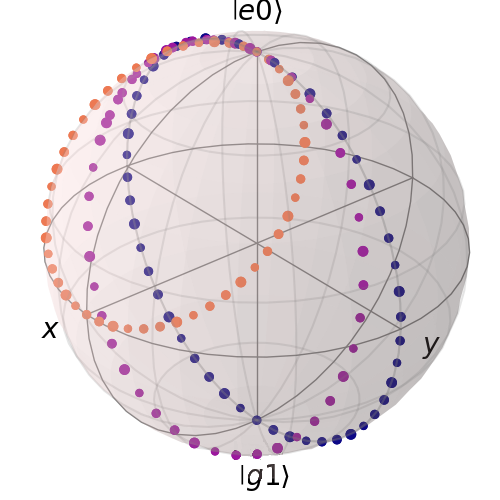
\includegraphics[width=\textwidth]{figuras/ch4/bloch eg0 bloch AC a=0 d=2.0 x=0.0 k=0.0 J=0.0 gamma=0.0 p=0.0.png}
    \end{minipage}\hfill
    \begin{minipage}[c]{0.3\textwidth}
        \caption{Trayectorias sobre la esfera de Bloch cuya condición inicial es $\ket{e_Ag_b0_C}$ para diferentes valores del detunning, apantallando el átomo B. Los valores son $\Delta=0$ (azul), $\Delta=0.5g$ (morada) y $\Delta=2g$ (naranja).}
        \label{fig4:bloch delta eg0}
    \end{minipage}
\end{figure}
Se observa como la dinámica entre estos dos estados es exactamente igual que la observada en la Figura \ref{fig3:bloch cinematica}, además, como todos los puntos están sobre la superficie de la esfera, los estados son puros y entonces el estado global es separable. Haber trazado sobre el átomo B no tuvo efecto sobre la dinámica entre el átomo A y la cavidad. Para corroborar esto se realiza un análisis poblacional más profundo.
Lo siguiente que se puede analizar, que no se tenía la posibilidad cuando se tiene 1 átomo, es considerar una condición inicial entrelazada. Si bien los átomos no interactúan (el átomo B está aislado del universo) se puede pensar que en algún momento los átomos se entrelazaron y luego se apagan las interacciones con el átomo B. Por ejemplo, si se considera el estado inicial entrelazado $\ket{\psi_0}=(\ket{eg0}+\ket{ge0})/\sqrt{2}$, se obtienen las trayectorias mostradas en la Figura \ref{fig4:bloch delta eg0 sim}.
\begin{figure}[H]
    \begin{minipage}[c]{0.67\textwidth}
        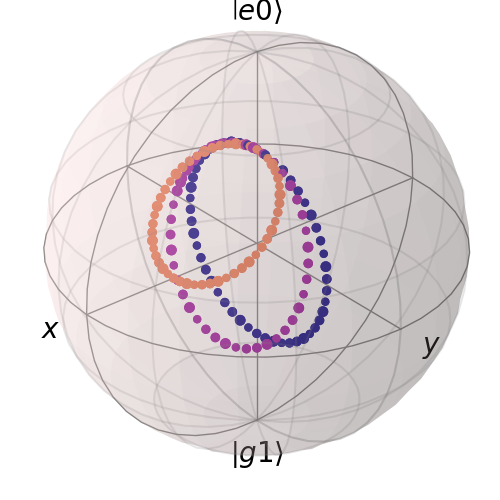
\includegraphics[width=\textwidth]{figuras/ch4/bloch eg0+ge0 bloch AC a=0 d=2.0 x=0.0 k=0.0 J=0.0 gamma=0.0 p=0.0.png}
    \end{minipage}\hfill
    \begin{minipage}[c]{0.3\textwidth}
        \caption{Trayectorias sobre la esfera de Bloch cuya condición inicial es $(\ket{e_Ag_b0_C}+\ket{g_Ae_b0_C})/\sqrt{2}$ para diferentes valores del detunning, apantallando el átomo B. Los valores son $\Delta=0$ (azul), $\Delta=0.5g$ (morada) y $\Delta=2g$ (naranja).}
    \end{minipage}
    \label{fig4:bloch delta eg0 sim}
\end{figure}
Ahora, los estados no están sobre la superficie, lo que se interpreta como que estamos en presencia de un estado mixto. Al trazar sobre el átomo B, efectivamente se considera como si este fuese parte de un entorno. Al olvidarse de la dinámica del segundo átomo, se puede interpretar como que este se lleva un 50\% de probabilidad de estar excitado, ya que no sabemos si inicialmente el átomo A o el átomo B es el que tiene la excitación. Entonces efectivamente tenemos un 50\% de probabilidad de que el estado de la cavidad sea $\ket{g0}$, y no evoluciona, y un 50\% de probabilidad de que la excitación este dentro de la cavidad, y por lo tanto vemos que la dinámica es la misma que en el caso anterior, pero con amplitudes menores.

Para analizar más en detalle la dinámica, y para poder realizar comparaciones cuando se complejiza el problema, se puede realizar un estudio poblacional, y también podemos mirar las entropías relativas y otros observables importantes.
En primer lugar, el caso separable $\psi_0=\ket{eg0}$, es idéntico al caso de 1 átomo, ya que el átomo B no evoluciona por estar totalmente aislado del sistema. Lo único que se puede resaltar es que, si se traza sobre la cavidad, que es algo útil para observar el entrelazamiento entre los átomos, entonces el estado es mixto, ya que la evolución temporal del sistema átomo A-átomo B consta del átomo B en el estado fundamental $\ket{g}$, y el átomo A oscila entre el estado excitado y fundamental. La amplitud de oscilación y el grado de \textit{mixing} entre los estados depende del detunning, siendo el caso $\Delta=0$ el de oscilaciones coherentes entre estados, y al aumentar $\Delta$ se atenúa este comportamiento.
En segundo lugar, cuando el estado inicial de los átomos no es separable por estar entrelazados $\ket{\psi_0}=(\ket{eg0} + \ket{ge0})/\sqrt{2}$, entonces la dinámica es un poco diferente. La figura \ref{fig4:dinamica eg0 sim resonante} muestra el caso de $\Delta=0$, donde se observan las evoluciones de las diferentes partes del sistema.

\begin{figure}[h]
    \centering
    \begin{subfigure}{0.49\textwidth}
        \centering
        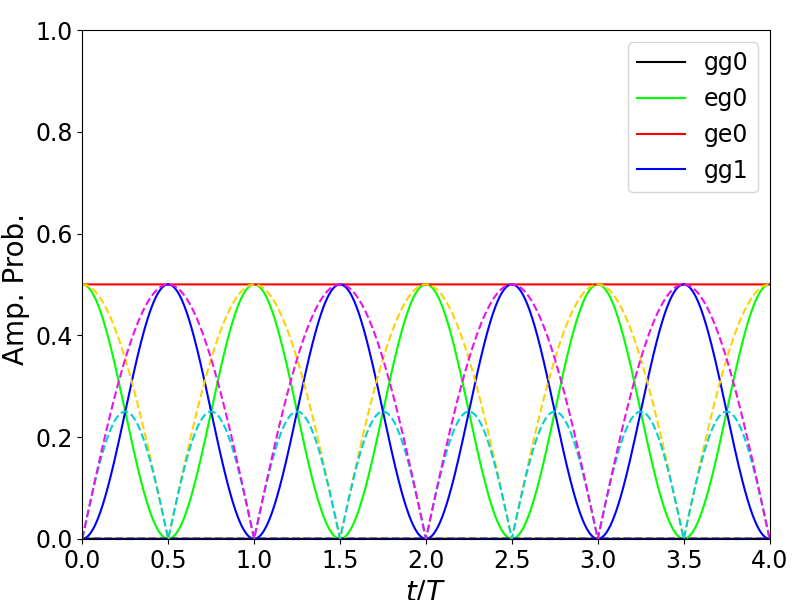
\includegraphics[width=\textwidth]{figuras/ch4/d eg0+ din ABC d=0.png}
        \caption{}
        \label{fig4:dinamica pob eg0 sim resonante}
    \end{subfigure}
    \hfill
    \begin{subfigure}{0.49\textwidth}
        \centering
        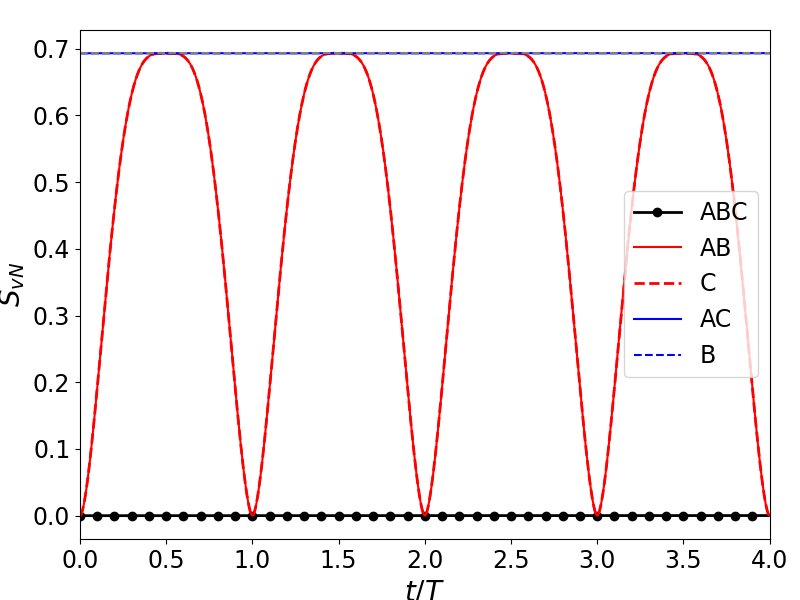
\includegraphics[width=\textwidth]{figuras/ch4/d eg0+ din svn d=0.png}
        \caption{}
        \label{fig4:dinamica svn eg0 sim resonante}
    \end{subfigure}
    \caption{\textcolor{red}{labels, ticks y legens chiquitos}(a):Dinámica poblacional para el caso resonante $\Delta=0$ con el estado inicial entrelazado $\ket{\psi_0}=(\ket{eg0} + \ket{ge0})/\sqrt{2}$. (b):Entropía de von Neuman del sistema total (negro con puntos), y de diferentes subsistemas. En rojo se muestra la entropía del sistema habiendo trazado parcialmente sobre la cavidad, y en azul habiendo trazado parcialmente sobre el átomo B.}
    \label{fig4:dinamica eg0 sim resonante}
\end{figure}

En la figura \ref{fig4:dinamica pob eg0 sim resonante} se muestran las poblaciones y las coherencias correspondientes a la condición inicial $\ket{\psi_0}=(\ket{eg0} + \ket{ge0})/\sqrt{2}$ en el caso resonante, y en la figura \ref{fig4:dinamica svn eg0 sim resonante} se muestra la entropía de Von Neuman, en función del tiempo $t/T$ con $T=2 \pi \Omega(n,j)$  . La entropía de von Neuman es una cantidad que está definida según:
\begin{equation}\label{ec4:entropia von neuman}
    S=-\Tr(\rho \ln \rho)=-\sum_j \lambda_j \ln \lambda_j,
\end{equation}
donde $\rho$ es la matriz densidad del sistema, y $\lambda_j$ son los autovalores de la matriz densidad. La entropía de Von Neuman sirve para determinar si un estado es puro o mixto, ya que $S(\rho)=0$ representa un estado puro, y $S(\rho)=\ln(N)$ representa un estado máximamente mixto, donde $N$ es la dimensión del espacio de Hilbert.
Vemos como el estado $\ket{ge0}$ no evoluciona, ya que en este caso, el átomo B contiene la única excitación y está aislado. Pero la otra parte, si que evoluciona. Vemos la presencia de las mismas oscilaciones coherentes entre los estados $\ket{eg0}$ y $\ket{gg1}$. La diferencia principal es que en este caso, el estado de los subsistemas es mixto. Esto se observa claramente en el gráfico de la entropía, pero también se puede deducir este comportamiento desde la Figura \ref{fig4:dinamica pob eg0 sim resonante}, ya que a $t/T=0.5$, tenemos el estado $\ket{\psi(T/2)}=\ket{g}_A\otimes(\ket{e_B0_C}+\ket{g_B1_C})/\sqrt{2}$, que es separable solo en el átomo A, y los otros dos están totalmente entrelazados, y por lo tanto al tomar traza parcial tal que el átomo B y la cavidad estén separadas, este estado es máximamente mixto. Vemos como el entrelazamiento entre la cavidad y el átomo B, que están totalmente aislados, evoluciona indirectamente por medio del átomo A, y paradójicamente este queda desentrelazado del sistema para tiempos $t=(k-1/2)T\; ; \; k \in \mathbb{N}$. En este punto notamos algo muy importante, y es que la entropía de von Neuman solo sirve para estados puros. Cuando $t=0$, la entropía del subsistema AB es 0, porque es un estado puro, y está máximamente entrelazado. Pero al evolucionar, el subsistema AB se hace mixto, y como se observa en la línea azul, la entropía del átomo B es siempre $\log 2$, que según la interpretación de la entropía de von Neuman es que está siempre máximamente entrelazado. Este no es al caso, y la descripción falla porque el estado AB no es puro.

Entonces, ya que el entrelazamiento es un recurso muy importante y estudiado para información cuántica, es necesario introducir una medida de entrelazamiento, para poder estudiarlo en este tipo de situaciones. Si bien la entropía de Von Neuman es útil en el caso de estados puros, cuando se tienen estados mixtos como se vio recién, o en el caso de tener un sistema abierto, esta medida ya no sirve. Una de las medidas más utilizadas y con mayor aplicación es el \textit{Entanglement of Formation} ($E_F$) \cite{Plenio2006}, que coincide con la entropía de von Neuman para estados puros, y sirve para estados mixtos. La $E_F$ está definida como
\begin{equation}
    E_F(\rho)=\text{inf}\left( \sum_i p_i E(\ketbra{\psi_i}{\psi_i}) : \rho = \sum_i p_i\ketbra{\psi_i}{\psi_i}\right)
\end{equation}
Esta medida representa el entrelazamiento promedio mínimo entre todas las posibles descomposiciones puras de $\rho$, donde $E(\ketbra{\psi_i}{\psi_i})=S(\tr_B{\ketbra{\psi_i}{\psi_i}})$ es la entropía de von Neuman, que es la medida que se utiliza para estados puros. Esta definición es general, pero en el caso presente, una simplificación de esta medida que se obtiene si se estudia el entrelazamiento entre dos qubits, como lo son los átomos A y B. Esta medida es la concurrencia, y está definida como
\begin{equation}
    C(\rho)=\text{max}\{0,\lambda_1-\lambda_2-\lambda_3-\lambda_4\},
    \label{ec4:concurrencia}
\end{equation}
donde los $\lambda_i$ son las raíces de los autovalores, en orden decreciente, de la matriz \newline $\rho(\sigma_y\otimes\sigma_y)\rho^*(\sigma_y\otimes\sigma_y)$, donde $\rho*$ es el conjugado (sin transponer) de $\rho$. La concurrencia y la entropía de formación $E_F$ están relacionadas, y la concurrencia obtiene su interpretación a través de esta. Un estado máximamente entrelazado tiene $C(\rho)=1$ y un estado separable $C(\rho)=0$. 


\begin{figure}[H]
    \begin{minipage}[c]{0.67\textwidth}
        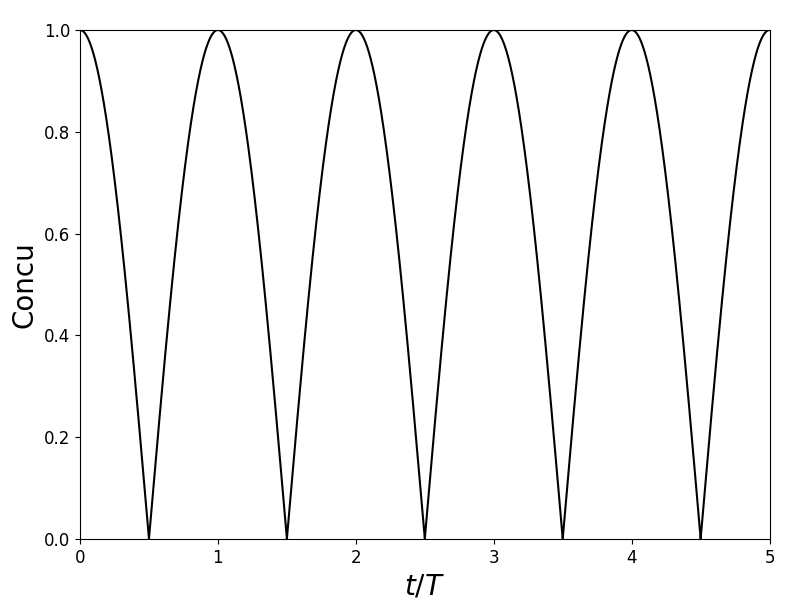
\includegraphics[width=\textwidth]{figuras/ch4/d eg0+ concu d=0.png}
    \end{minipage}\hfill
    \begin{minipage}[c]{0.3\textwidth}
    \caption{Concurrencia en el caso resonante para estado inicial $\ket{eg0}+\ket{ge0}$} 
    \label{fig4:concu eg0 sim}
  \end{minipage}
\end{figure}
En la figura \ref{fig4:concu eg0 sim} se observa la concurrencia entre los átomos AB, para el caso estudiado anteriormente. Como era de esperar, a $t=0$ el estado es máximamente entrelazado, y luego el entrelazamiento se pierde a $t=T/2$, donde el átomo B está entrelazado con la cavidad. 

\subsection{Interacción átomo-átomo}

El siguiente paso es analizar el rol de las interacciones entre los átomos, aún manteniendo el apantallamiento $\alpha=0$. Para esto, se sigue utilizando las mismas condiciones iniciales y el átomo B seguirá sin interactuar con la cavidad, pero se considera ahora que la interacción entre átomos dadas por los parámetros $k$ y $J$ serán distintos de cero. Para comenzar, en la figura \ref{fig4:k eg0 abc} se observa la evolución temporal para el estado inicial $\ket{\psi_0}=\ket{eg0}$, con $\Delta = 0$, $J=0$ pero $k=0.1g$. Recordar que $k$ es la intensidad de la interacción $\sigma^{(1)}_+\sigma^{(2)}_-+\text{c.c.}$ (ver Ec. (\ref{ec4:H})).

\begin{figure}[h]
    \begin{minipage}[c]{0.67\textwidth}
        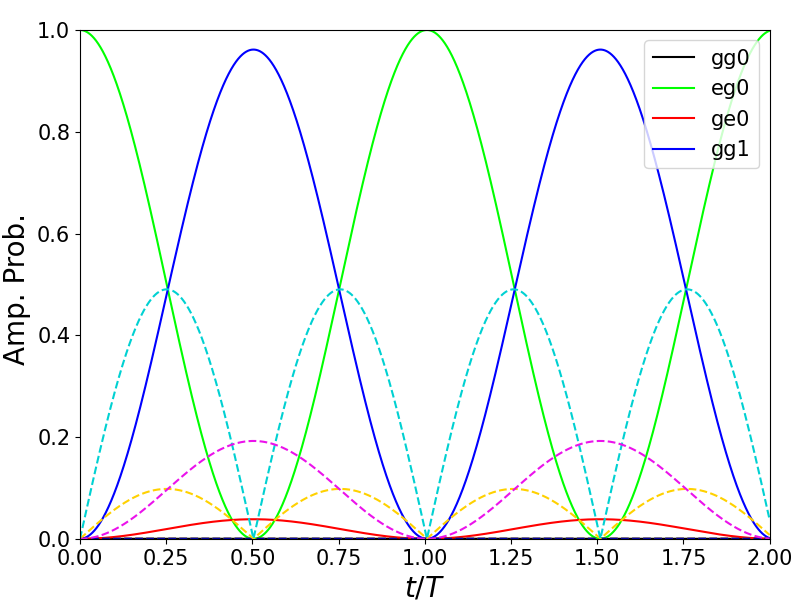
\includegraphics[width=\textwidth]{figuras/ch4/k eg0 ABC.png}
    \end{minipage}\hfill
    \begin{minipage}[c]{0.3\textwidth}
    \caption{Dinámica poblacional para la condición inicial $\ket{\psi_0}=\ket{eg0}$, para los parámetros $\Delta=0$, $J=0$ y $k=0.1g$. Las líneas solidas se corresponden con las poblaciones de la matriz densidad total del sistema; en azul la probabilidad de encontrar al estado en el estado $\ket{gg1}$, en verde en $\ket{eg0}$, en rojo $\ket{ge0}$, y en negro $\ket{gg0}$. Las líneas rayadas son las coherencias entre estas poblaciones, la violeta entre $\ket{gg1}$ y $\ket{ge0}$, la celeste entre $\ket{eg0}$ y $\ket{gg1}$ y la amarilla entre $\ket{eg0}$ y $\ket{gg1}$.
         } \label{fig4:k eg0 abc}
  \end{minipage}
\end{figure}
Lo que sucede es que la excitación está inicialmente en el átomo A, y como siempre, se observan oscilaciones entre los estados $\ket{eg0}$ y $\ket{gg1}$, la diferencia es que al haber interacciones entre los átomos, ahora la excitación inicial que está en el átomo A, sufre dos procesos diferentes, primero la oscilación, y además, la interacción con el átomo B. Al tener la excitación el átomo A, una parte de esta se va hacia la cavidad, y la otra hacia el átomo B, excitándolo parcialmente. La amplitud de la oscilación depende de la intensidad de la interacción $k$. Mediante la curva roja, se contempla que su pendiente crece mientras que la probabilidad de $\ket{eg0}$ es mayor a la de $\ket{gg1}$. Cuando las probabilidades cambian, la amplitud crece, pero de manera desacelerada, hasta que la probabilidad del estado $\ket{eg0}$ es nula. En ese momento, ya no hay excitación que pasar del átomo A al B, y el proceso se revierte. Antes de analizar el entrelazamiento entre los átomos, se observa en la Figura \ref{fig4:k eg0 sim abc} la dinámica para los mismos parámetros, pero para la condición inicial entrelazada $\ket{\psi_0}=(\ket{eg0}+\ket{ge0})/\sqrt{2}$:
\begin{figure}[h]
    \begin{minipage}[c]{0.67\textwidth}
        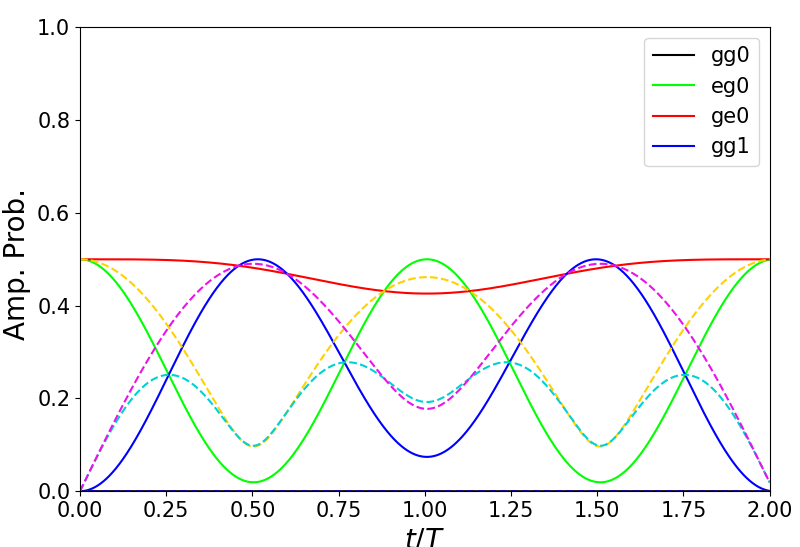
\includegraphics[width=\textwidth]{figuras/ch4/k eg0+ ABC.png}
    \end{minipage}\hfill
    \begin{minipage}[c]{0.3\textwidth}
    \caption{Dinámica poblacional para la condición inicial $\ket{\psi_0}=\ket{eg0+ge0}$, para los parámetros $\Delta=0$, $J=0$ y $k=0.1g$. Las coherencias y poblaciones tienen los mismos colores que la Figura anterior \ref{fig4:k eg0 abc}}
    \label{fig4:k eg0 sim abc}
  \end{minipage}
\end{figure}
La dinámica en este caso presenta oscilaciones en la población de $\ket{ge0}$ con un periodo dos veces más grande. Esto se debe a una \textit{pelea} entre los estados $\ket{eg0}$ y $\ket{ge0}$, ya que tienen las excitaciones en diferentes átomos. Inicialmente, como los estados están entrelazados, no está bien definido en cuál de los dos átomos está la excitación, entonces la interacción $k$ se anula y la curva tiene pendiente 0. Entonces la dinámica inicial es igual que para $k=0$ y comienza a oscilar. Al decrecer la curva verde, la probabilidad de encontrar la excitación en el átomo B es mayor que la del átomo A, entonces el átomo B comienza a perder esta excitación y se la da lentamente al átomo A, y por lo tanto la oscilación del estado $\ket{eg0}$ no llega a tener amplitud nula en $t/T=0.5$. Luego, la evolución sigue su curso oscilante, y al llegar a $t=T$, la probabilidad de encontrar la excitación en el átomo A es mayor que en el átomo B, y por lo tanto comienza a revertirse la situación, hasta completar el ciclo para $t=2T$. 

El entrelazamiento entre los átomos se analiza utilizando la concurrencia, como se muestra en la figura \ref{fig4:concu k}, donde \ref{fig4:concu k eg0} muestra la condición inicial separable $\ket{eg0}$, y \ref{fig4:concu k eg0 sim} el entrelazamiento para la condición inicial entrelazada $\ket{eg0+ge0}$. 
\begin{figure}[h]
    \centering
    \begin{subfigure}{0.49\textwidth}
        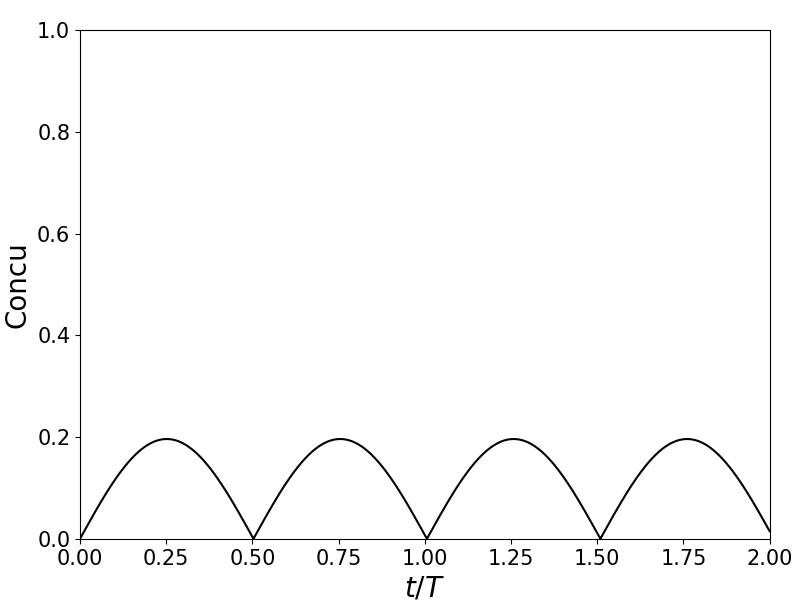
\includegraphics[width=\textwidth]{figuras/ch4/k eg0 concu.png}
        \caption{$\ket{eg0}$}
        \label{fig4:concu k eg0}
    \end{subfigure}
    \hfill
    \begin{subfigure}{0.49\textwidth}
        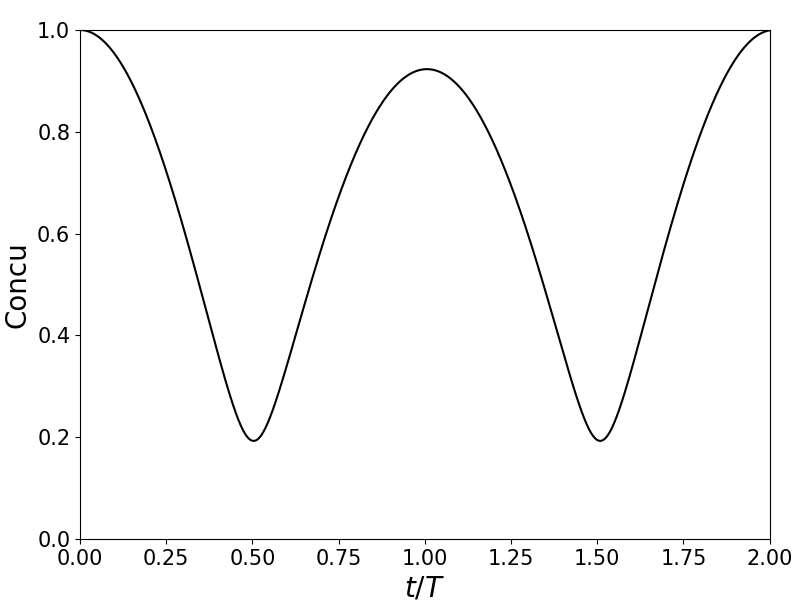
\includegraphics[width=\textwidth]{figuras/ch4/k eg0+ concu.png}
        \caption{$\ket{eg0+ge0}$}
        \label{fig4:concu k eg0 sim}
    \end{subfigure}
    \caption{Dinámica de entrelazamiento para $\Delta=0$, $J=0$ y $k=0.1g$}
    \label{fig4:concu k}
\end{figure}

Ahora se analiza la interacción tipo Ising, para eso se utilizan parámetros $k=0$ y $J\neq 0$. En la figura \ref{fig4:j alpha0} se observa que, si bien la dinámica es similar, los átomos no se entrelazan.

\begin{figure}[H]
    \centering
    \begin{subfigure}{0.49\textwidth}
        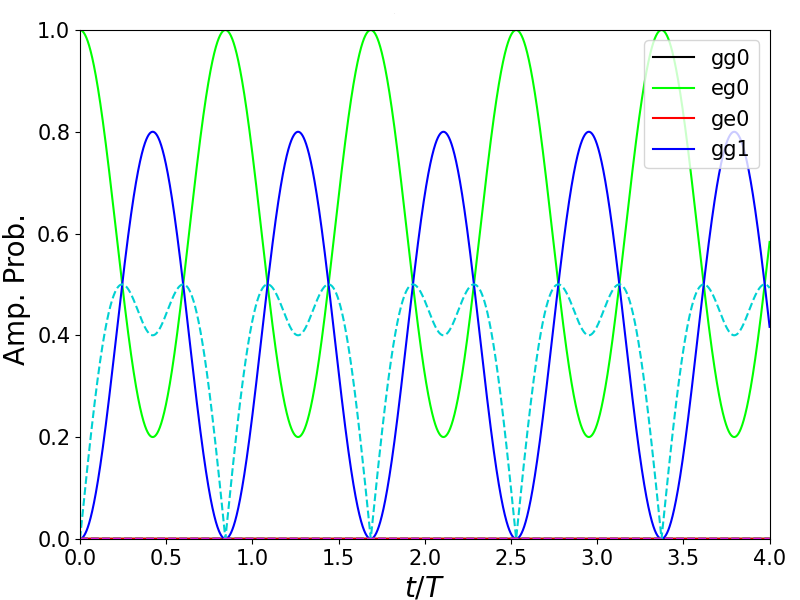
\includegraphics[width=\textwidth]{figuras/ch4/j eg0 abc.png}
        \caption{$\ket{eg0}$ Poblaciones}
        \label{fig4:pob j eg0}
    \end{subfigure}
    \hfill
    \begin{subfigure}{0.49\textwidth}
        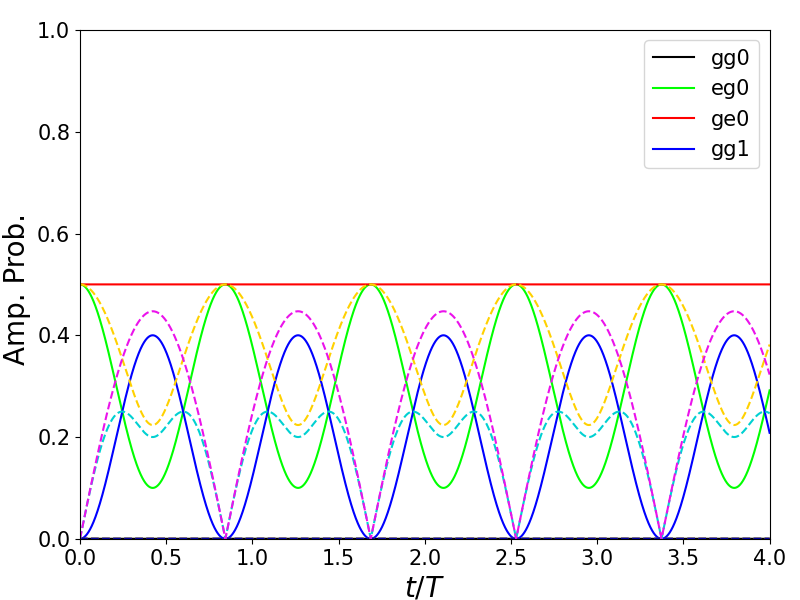
\includegraphics[width=\textwidth]{figuras/ch4/j eg0+ge0 abc.png}
        \caption{$\ket{eg0+ge0}$ Poblaciones}
        \label{fig4:pob j eg0 sim}
    \end{subfigure}
    \vfill
    \begin{subfigure}{0.49\textwidth}
        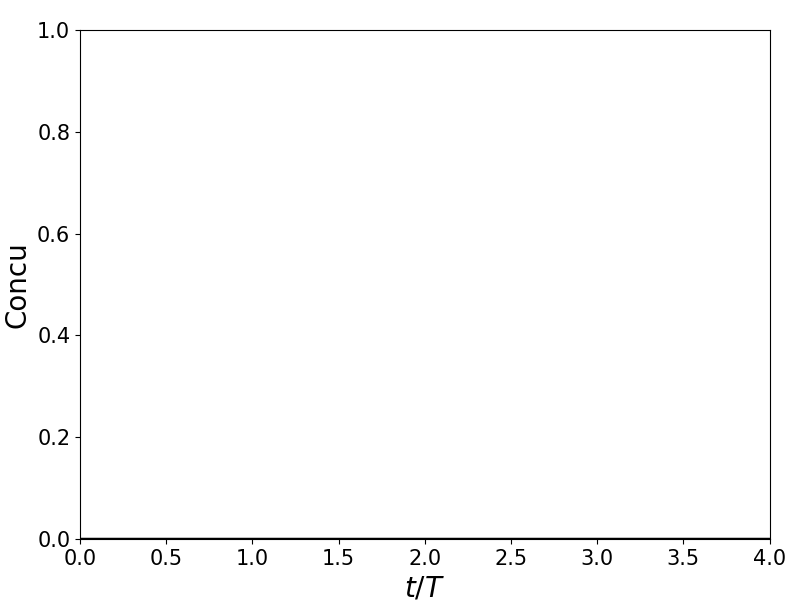
\includegraphics[width=\textwidth]{figuras/ch4/j eg0 concu.png}
        \caption{$\ket{eg0}$ Concurrencia}
        \label{fig4:pob j eg0}
    \end{subfigure}
    \hfill
    \begin{subfigure}{0.49\textwidth}
        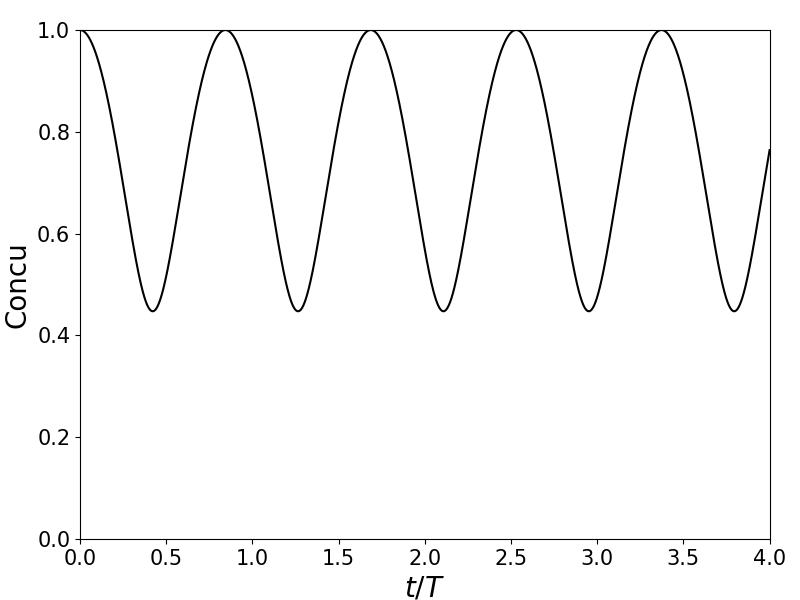
\includegraphics[width=\textwidth]{figuras/ch4/j eg0+ge0 concu.png}
        \caption{$\ket{eg0+ge0}$ Concurrencia}
        \label{fig4:pob j eg0 sim}
    \end{subfigure}
    \caption{$\Delta=0$, $J=0.5g$ y $k=0$}
    \label{fig4:j alpha0}
\end{figure}
La diferencia principal entre la interacción tipo Isign ($J\sigma_z^{(1)}\sigma_z^{(2)}$) y la dipolar ($k\sigma_+^{(1)}\sigma_-^{(2)}+\text{c.c.}$), es que el segundo parece entrelazar los átomos, ya que en el primer caso, el efecto es separar los niveles de energía, pero en el segundo no solo eso, sino que también pasa excitaciones de un átomo al otro. Si bien esto sirve para entender intuitivamente el efecto, el problema de este análisis es que se asumen cosas no físicas mediante el apantallamiento y la asimetría que se impone entre los dos átomos. Ya que en el Hamiltoniano del sistema sin apantallamiento (Ec. (\ref{ec4:H})), donde se utiliza la base con estados simétricos y antisimétricos (Ec. (\ref{ec4:base})), el efecto de ambos parámetros debería ser el mismo, ya que solo aparecen en la diagonal principal. Si bien la interacción $J$ actúa sobre todos los estados, y el $k$ solamente solo sobre los $\ket{egn\pm gen}$, su principal función es separar las energías de los estados de la base.
Entonces será necesario retomar este análisis sin apantallamiento y con la base adecuada de la Ec.(\ref{ec4:base}).
\subsection{Medio Kerr}
\label{sec4:medio kerr}
Ahora se enfoca el estudio del efecto del medio Kerr. Para esto, se apagan las interacciones interatómicas $k=J=0$, y se modifica la no linealidad medio a través del parámetro $\chi$. 
\begin{figure}[h]
    \centering
    \begin{subfigure}{0.49\textwidth}
        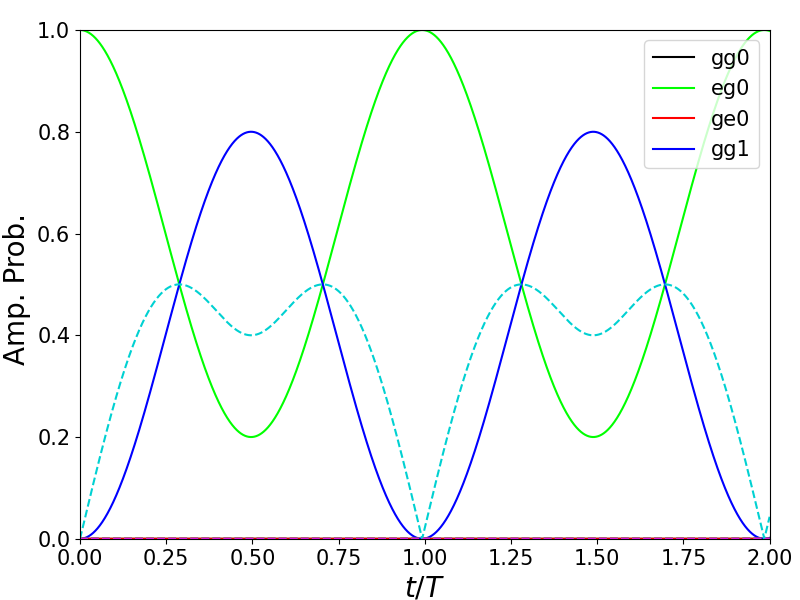
\includegraphics[width=\textwidth]{figuras/ch4/x eg0 abc.png}
        \caption{$\ket{eg0}$}
        \label{fig4:pob x eg0}
    \end{subfigure}
    \hfill
    \begin{subfigure}{0.49\textwidth}
        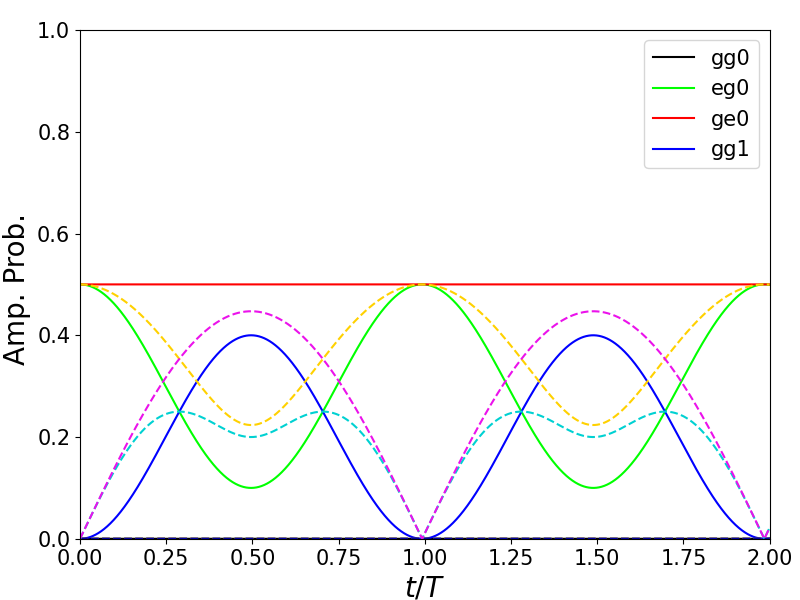
\includegraphics[width=\textwidth]{figuras/ch4/x eg0+ abc.png}
        \caption{$\ket{eg0+ge0}$}
        \label{fig4:pob x eg0 sim}
    \end{subfigure}
    \caption{Dinámica de poblaciones para $x=g$}
    \label{fig4:pob x}
\end{figure}

Al igual que en el caso de 1 átomo, se puede observar en las Ec. (\ref{ec4:autoenergias}) y Ec. (\ref{ec4:parametros solucion}) que la frecuencia depende del medio. En la Figura \ref{fig4:pob x} el tiempo está normalizado con la frecuencia, entonces no se nota el cambio. Pero lo que es necesario analizar, es como las oscilaciones no son totalmente coherentes, en el sentido de que la amplitud de probabilidad no es 1, como en el caso de $\chi=0$. Esto se debe a que el aumento de $\chi$ hace que las energías de ambos estados se separen, y por lo tanto hace que las transiciones entre los estados sea menos probable. Este comportamiento también se observa si el estado inicial se toma como $\ket{gg1}$. Es lógico estudiar el entrelazamiento en este caso. En la Figura \ref{fig4:concu x} se muestran las concurrencias para ambas condiciones iniciales. Es interesante comparar la Figura \ref{fig4:concu x eg0 sim} con la figura en el caso de $\chi=0$ para esta misma condición inicial representada en la Figura \ref{fig4:concu eg0 sim}. En principio se puede pensar que el medio no lineal rompe con el entrelazamiento del sistema, pero como se ve al comparar estas figuras, la interpretación correcta es que el medio no hace más que ralentizar el comportamiento preexistente de la cavidad, ya que en este caso, no destruye el entrelazamiento, sino que lo conserva por virtud de haber ralentizado las amplitudes de oscilación entre los dos estados dinámicos.
\begin{figure}[h]
    \centering
    \begin{subfigure}{0.49\textwidth}
        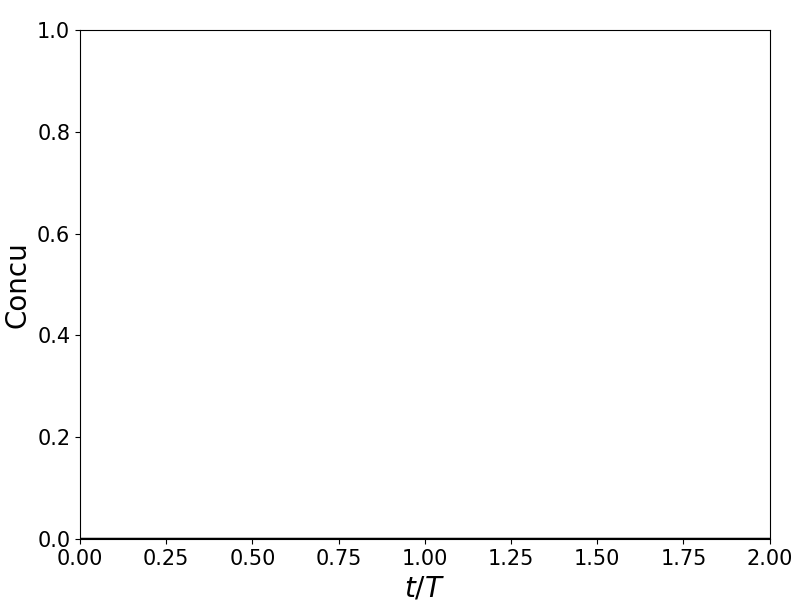
\includegraphics[width=\textwidth]{figuras/ch4/x eg0 concu.png}
        \caption{$\ket{eg0}$}
        \label{fig4:concu x eg0}
    \end{subfigure}
    \hfill
    \begin{subfigure}{0.49\textwidth}
        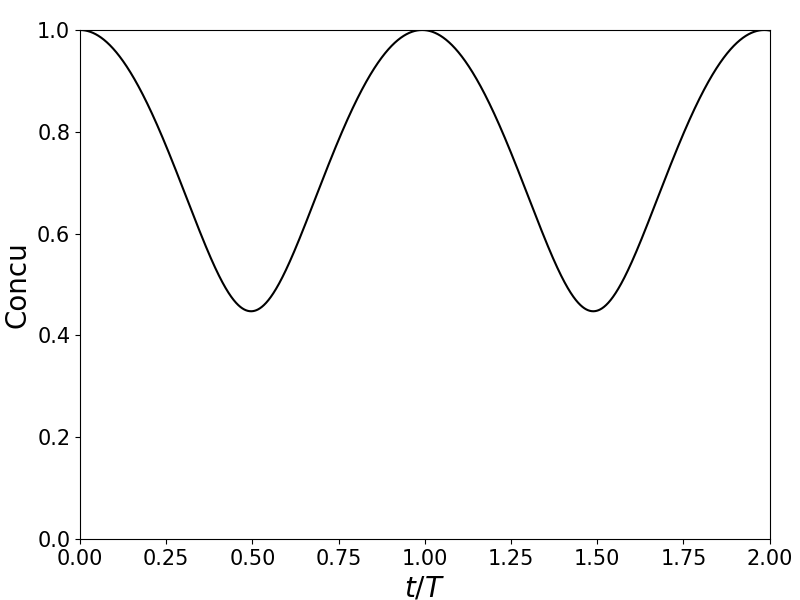
\includegraphics[width=\textwidth]{figuras/ch4/x eg0+ concu.png}
        \caption{$\ket{eg0+ge0}$}
        \label{fig4:concu x eg0 sim}
    \end{subfigure}
    \caption{Dinámica de entrelazamiento para $x=g$}
    \label{fig4:concu x}
\end{figure}
También se puede recuperar el comportamiento visto en el modelo de 1 átomo, que el medio Kerr no es más que un desplazamiento lateral en las frecuencias, además de modificar las amplitudes. Para esto se realiza otra evolución para $\chi=\Delta=\frac{g}{2}$, y se compara con el caso en que $\chi=\Delta=0$
\begin{figure}[h]
    \centering
    \begin{subfigure}{0.49\textwidth}
        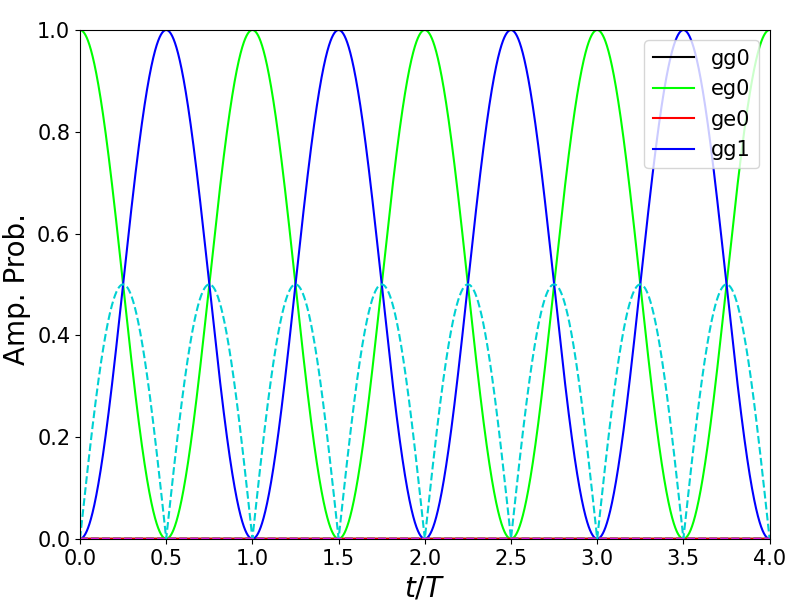
\includegraphics[width=\textwidth]{figuras/ch4/d=x=0 eg0 abc.png}
        \caption{$\Delta=\chi=0$}
        \label{fig4:comparacion kerr pob 1}
    \end{subfigure}
    \hfill
    \begin{subfigure}{0.49\textwidth}
        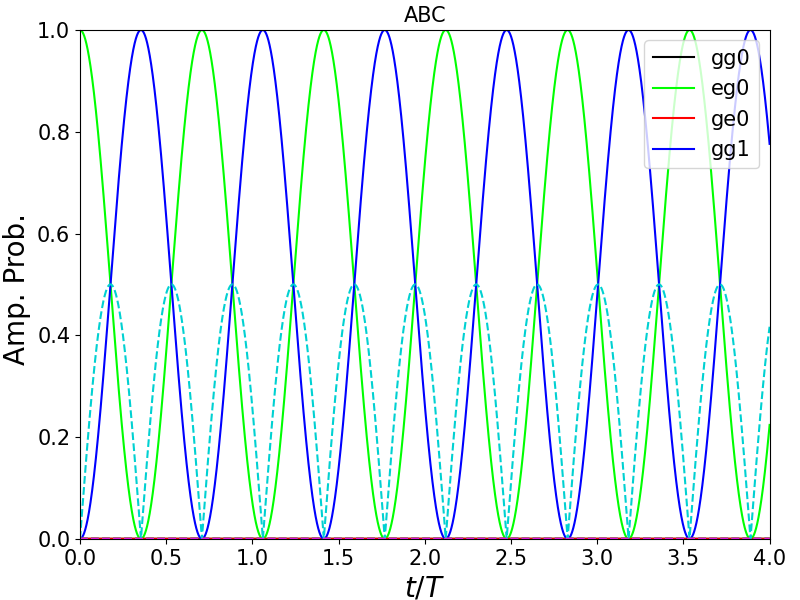
\includegraphics[width=\textwidth]{figuras/ch4/d=x=0.5 eg0 abc.png}
        \caption{$\Delta=\chi=0.5g$}
        \label{fig4:comparacion ker pob 2}
    \end{subfigure}
    \caption{Dinámica de entrelazamiento para $x=g$}
    \label{fig4:comparacion d vs x}
\end{figure}
Se observa como se anula el efecto del medio, y la dinámica es la misma pero con un cambio en la frecuencia. Al igual que antes, aumenta la frecuencia.

\subsection{Batidos}

Al complejizar el problema, la dinámica comienza a presentar batidos entre las amplitudes de probabilidad de las poblaciones y en las coherencias, comportamiento que se atribuye a la modulación de dos procesos simultáneos. Por ejemplo, en la evolución temporal con $\chi\neq0$ y $k\neq0$, entonces el primero disminuye la amplitud de oscilación de los estados con mayor cantidad de fotones en la cavidad, que dentro del subespacio $N$ la jerarquía del medio sera favorecer a los estados $\ket{eg,N-1}$ y $\ket{ge,N-1}$ por sobre el $\ket{ggN}$. Por el contrario, se observó que en esta situación, el término de interacción entre los átomos disminuye la amplitud del estado $\ket{ggN}$ como se vio en la sección anterior. Por lo tanto, si dos procesos están en juego y sus efectos son similares, entonces es esperable que se observen oscilaciones moduladas. No vale la pena mostrar la dinámica de las poblaciones, porque no se pueden sacar conclusiones muy importantes, pero sí podemos observar la trayectoria en la esfera de Bloch, para dar una idea de la complejidad de la evolución.
\begin{figure}[h]
    \centering
    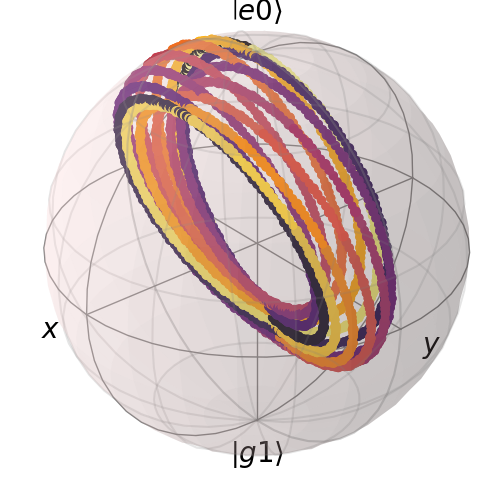
\includegraphics[width=0.5\linewidth]{figuras/ch4/eg0 bloch AC a=0 d=0.0 x=0.5 k=0.5 J=0.0 gamma=0.0 p=0.0.png}
    \caption{Trayectoria sobre la esfera de Bloch para el estado inicial $\ket{eg0}$, trazando parcialmente sobre el átomo B, y los parámetros utilizados son $\Delta=0$,$\chi=0.5g$,$k=0.5g$ y $J=0$.}
    \label{fig4:eg0 bloch batidos}
\end{figure}
En la Figura \ref{fig4:eg0 bloch batidos} se representa la trayectoria en el espacio de estados cuyo estado inicial es $\ket{eg0}$, habiendo trazado parcialmente sobre el átomo B que está apantallado. Es evidente por la curva descrita en la bola de Bloch, que la dinámica es complicada y los análisis poblacionales carecen de sentido, ya que se pierde la periodicidad y se complejizan las interpretaciones. En este gráfico, el color representa el tiempo comenzando por el color negro, y aclarándose hasta llegar a $t=7T$ representado por el color amarillo. 
\section{Dinámica sin apantallamiento}
\label{sec4:dinamica sin apantallamiento}

Al sacar el apantallamiento, es necesario utilizar la base de la Ec. (\ref{ec4:base}), ya que los átomos son indistinguibles y esta base es más apropiada. Además, el Hamiltoniano desacopla los estados antisimétricos, facilitando la solución. Por lo tanto, se procede a estudiar la dinámica sacando el apantallamiento. Resulta de interés estudiar el entrelazamiento entre los átomos, y su dependencia con los parámetros. 

\subsection{Dinámica con disipación}
Para modelar la dinámica disipativa se utiliza nuevamente el formalismo de la ecuación de Lindblad, donde los operadores de colapso ahora deben tener en cuenta a ambos átomos por igual. Se consideran los procesos de pérdidas al igual que en el caso de un átomo como la pérdida de fotones por las imperfecciones de la cavidad, y el bombeo incoherente de los átomos. La ecuación maestra ahora tiene los operadores

\begin{align}
    L_\gamma&=\sqrt{\gamma}\hat a, \\
    L_p &=\sqrt{p}(\hat\sigma_+^{(1)}+\hat\sigma_+^{(2)}).  
\end{align}

Lo primero que hay que considerar es la dependencia de la dinámica con el régimen de acoplamiento, se espera un comportamiento igual al del caso de un átomo (sección \ref{sec3:regimen acoplamiento}). Recordar que el régimen de acoplamiento fuerte (SC) es el caso en donde la interacción entre cavidad y átomos es mayor a la interacción entre sistema y entorno.
\begin{figure}[h]
    \centering
    \begin{subfigure}{0.7\textwidth}
        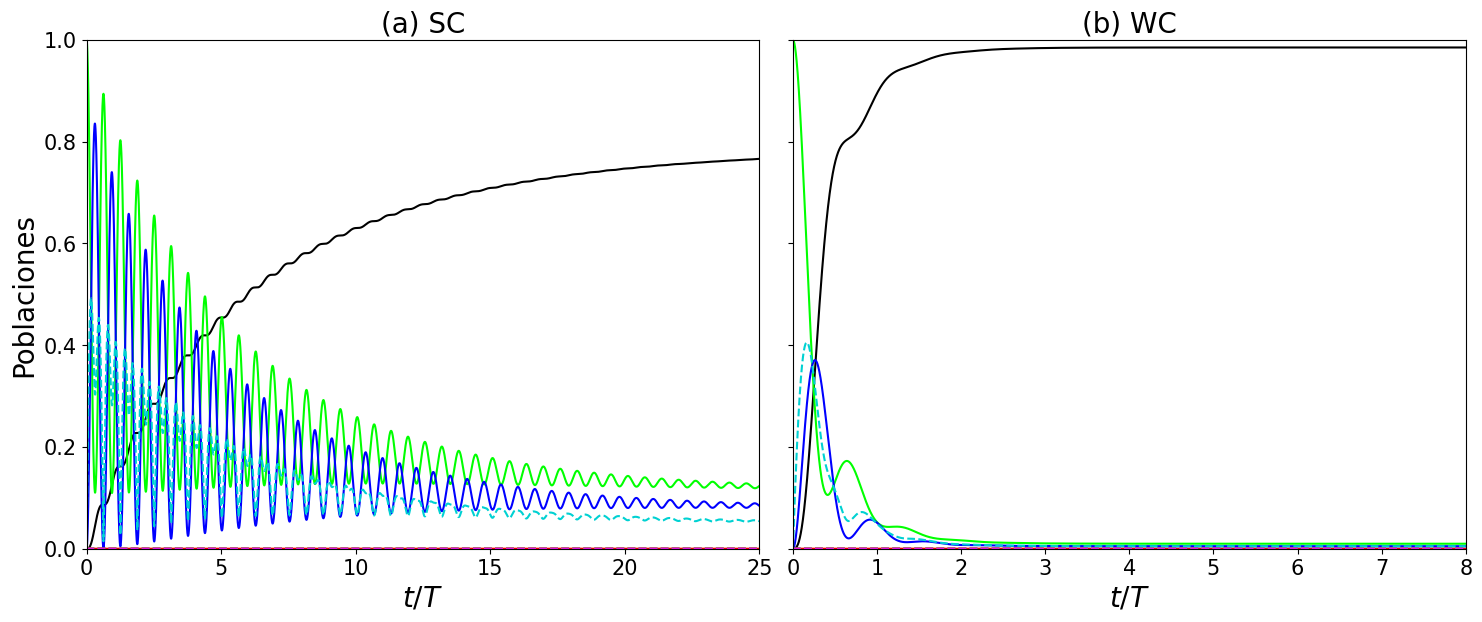
\includegraphics[width=\textwidth]{figuras/ch4/sc vs wc eg0 sim j0.5.png}
        \caption{}
        \label{fig4:acoplamiento eg0 sim}
    \end{subfigure}
    \vfill
    \begin{subfigure}{0.7\textwidth}
        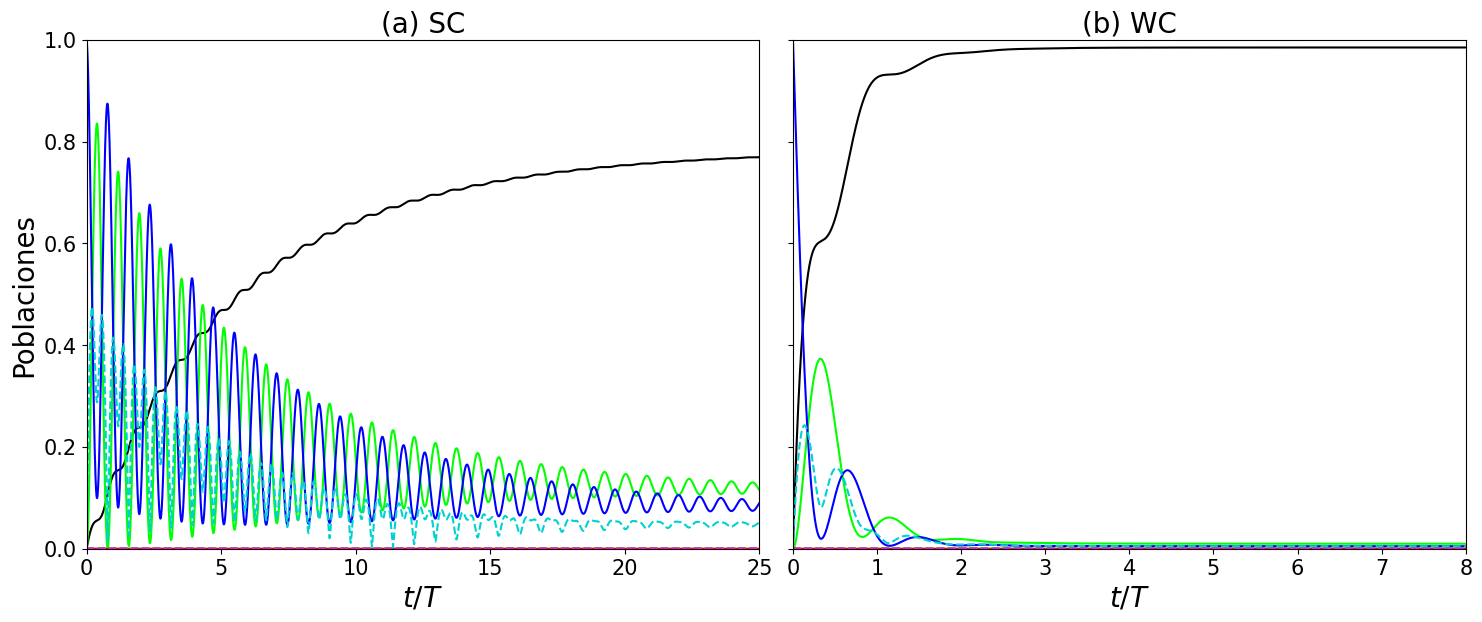
\includegraphics[width=\textwidth]{figuras/ch4/sc vs wc gg1 k=0.5.png}
        \caption{}
        \label{fig4:acoplamiento gg1}
    \end{subfigure}
    \caption{Dependencia de las poblaciones con el régimen de acoplamiento, para $\Delta=J=\chi=0$ y $k=0.5g$, y para dos condiciones iniciales diferentes. (a) $\ket{eg0+ge0}$, $\Delta=\chi=k=0$, $J=0.5g$; (b) $\ket{gg1}$, $\Delta=\chi=J=0$, $k=0.5g$.}
    \label{fig4:regimen acoplamiento}
\end{figure}
En  la figura \ref{fig4:regimen acoplamiento} se muestran las coherencias y las poblaciones, como se esperaba, estas tienen el mismo comportamiento que en el caso de 1 átomo. Notablemente, se puede ver el efecto de la interacción entre los átomos, como se separan las energías inicialmente las oscilaciones no logran la inversión total de población, solo una inversión parcial, y a tiempos largos la disipación hace que se tenga una mayor probabilidad de encontrar al sistema en el estado $\ket{eg0+ge0}$ ya que tiene menor energía. Eventualmente alcanza su estado estacionario. Lo que se recupera, ahora que ya no hay apantallamiento, es que ambos tipos de interacción ($J$ y $k$) generan entrelazamiento, consecuentemente la concurrencia para ambas interacciones es oscilante.

Nuevamente, nos concentraremos en el régimen SC. Si bien hasta ahora se estudió principalmente estados con 1 excitación, interesantes por sus implicancias y similitudes al modelo de 1 átomo, considerar estados con mayor cantidad de excitaciones hace a la riqueza del problema. Si solo consideramos $N=1$, el subespacio del problema tiene 3 estados, de los cuales uno es el estado antisimetrico $\ket{eg0-ge0}$ que está desconectado de los otros estados, y por lo tanto efectivamente se tiene un modelo de Jaynes-Cummings de 1 atomo con 2 estados dinamicamente relevantes. Si se permiten $N=2$ excitaciones, ahora hay 4 estados en el subespacio, de los cuales 3 son relevantes. Primero veremos cuales son los efectos de las interacciones y la dinámica para estados iniciales en el subespacio de $N=2$. Para mantener el paralelismo, comenzaremos con el estado $\ket{eg1+ge1}$, pero como se verá, las condiciones iniciales cambian totalmente la dinámica de entrelazamiento del sistema. La enorme cantidad de posibilidades para elegir condiciones iniciales, hace que estudiar todos sea imposible, así que se  concentrarán los esfuerzos en algunos de ellos.
Al tener 3 estados dinámicamente relevantes, se tienen 3 autoestados con sus respectivas autoenergías, y por lo tanto 3 frecuencias que compiten entre si, y son las 3 frecuencias de Rabi del sistema:
\begin{equation}
    \begin{aligned}
        \Omega^{(n)}_{12} &= E^{(n)}_2-E^{(n)}_1 ,\\
        \Omega^{(n)}_{23} &=E^{(n)}_3-E^{(n)}_2, \\
        \Omega^{(n)}_{31} &= E^{(n)}_1-E^{(n)}_3 .        
    \end{aligned}
    \label{ec4:frecuencias de rabi}
\end{equation}
Estas frecuencias se muestran en función del detunning $\Delta$ y para diferentes valores de $\chi$ y de $k-J$ en la figura \ref{fig4:frecuencias de rabi}.
\begin{figure}
    \centering
    \begin{subfigure}{0.49\textwidth}
        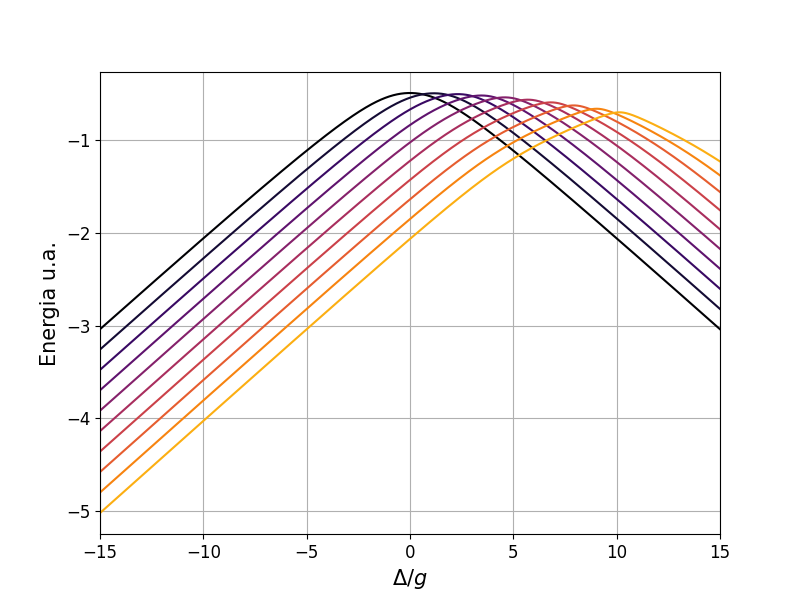
\includegraphics[width=\textwidth]{figuras/ch4/omega12 2d chi.png}
        \caption{}
        \label{fig4:rabi 1 chi}
    \end{subfigure}
    \hfill
    \begin{subfigure}{0.49\textwidth}
        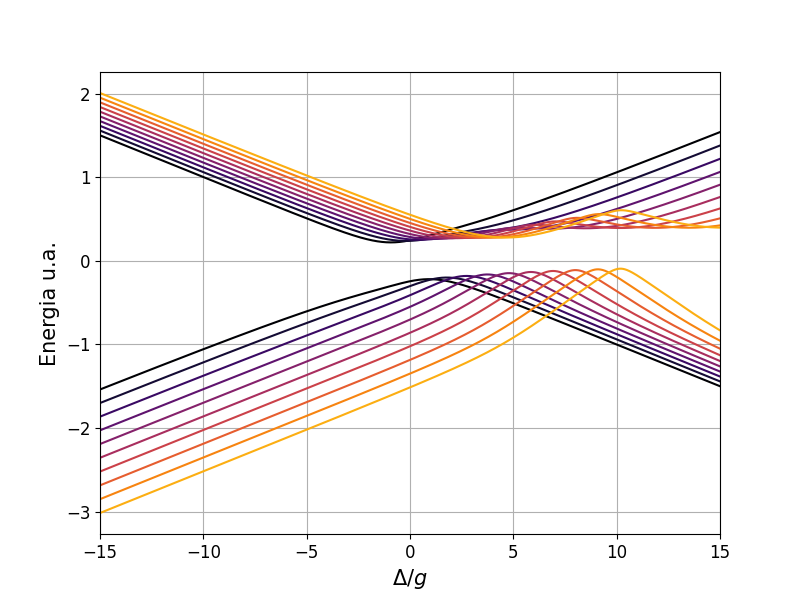
\includegraphics[width=\textwidth]{figuras/ch4/omega23 2d chi.png}
        \caption{}
        \label{fig4:rabi 2 chi}
    \end{subfigure}
    \vfill
    \begin{subfigure}{0.49\textwidth}
        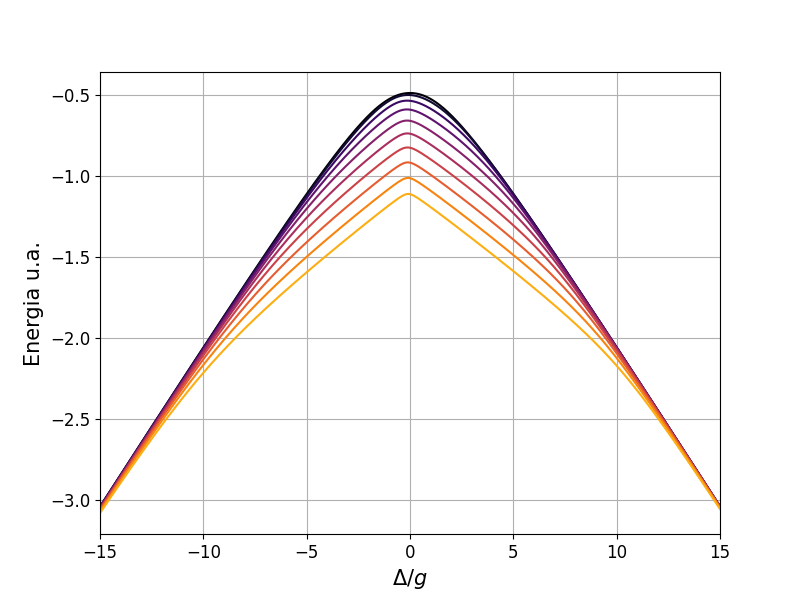
\includegraphics[width=\textwidth]{figuras/ch4/omega12 2d k.png}
        \caption{}
        \label{fig4:rabi 1 k}
    \end{subfigure}
    \hfill
    \begin{subfigure}{0.49\textwidth}
        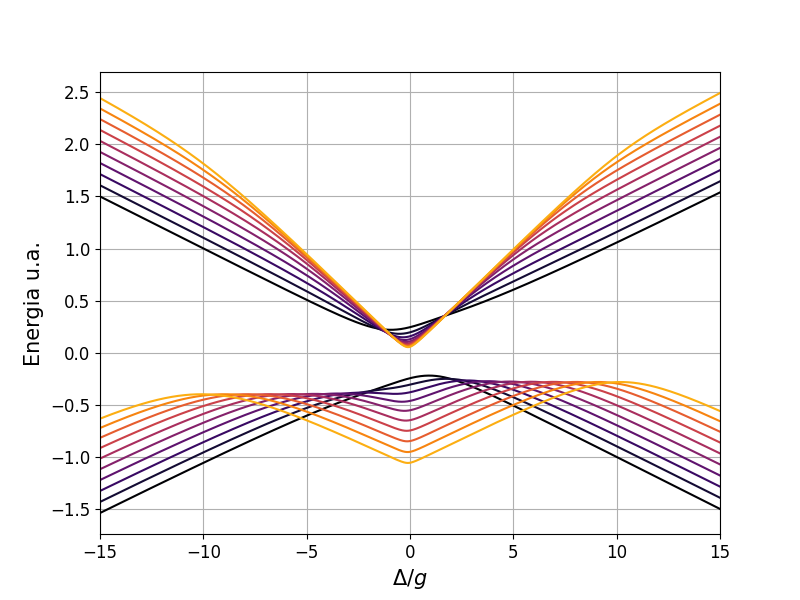
\includegraphics[width=\textwidth]{figuras/ch4/omega23 2d k.png}
        \caption{}
        \label{fig4:rabi 2 k}
    \end{subfigure}
    \caption{Frecuencias de Rabi en función del detunning $\Delta$ para diferentes valores de $\chi$, y $|k-J|$, donde las frecuencias de Rabi son $\Omega^{(2)}_{ij}=E^{(2)}_{j}-E^{(2)}_{i}$. (a) $\Omega_{12}$ con $\chi\in [0,5g]$; (b) $\Omega_{23}$ y $\Omega_{31}$ con $\chi\in [0,5g]$ ;(c) $\Omega_{12}$ con $k-J\in [0,5g]$ ; (d) $\Omega_{23}$ y $\Omega_{31}$ con $k-J\in [0,5g]$}
    \label{fig4:frecuencias de rabi}
\end{figure}


% \begin{figure}
%     \centering
%     \begin{subfigure}{0.3\textwidth}
%         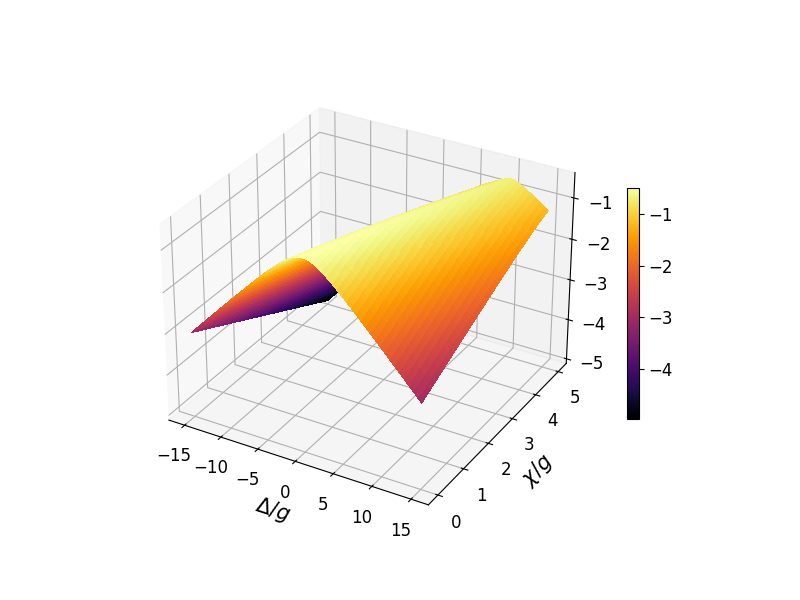
\includegraphics[width=\textwidth]{figuras/ch4/omega12 k=0.png}
%         \caption{}
%         \label{fig4:rabi chi}
%     \end{subfigure}
%     \hfill
%     \begin{subfigure}{0.3\textwidth}
%         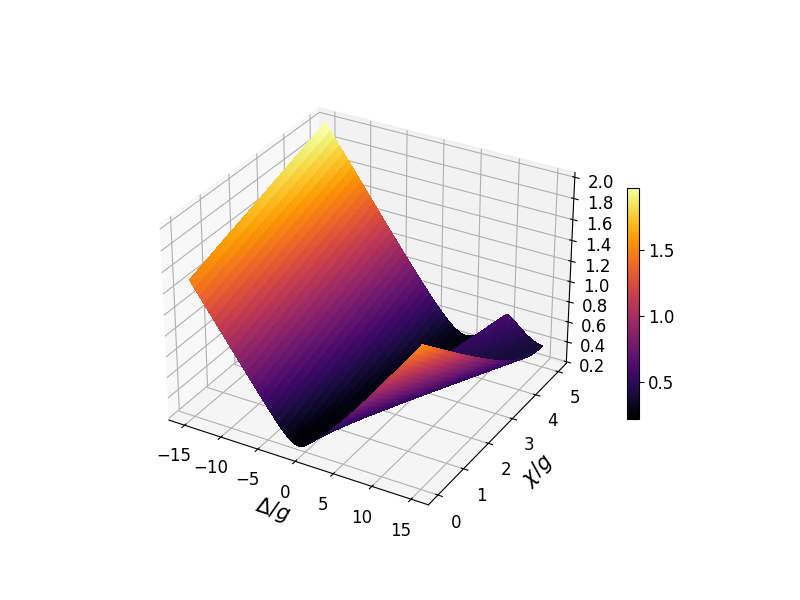
\includegraphics[width=\textwidth]{figuras/ch4/omega23 k=0.png}
%         \caption{}
%         \label{fig4:rabi chi}
%     \end{subfigure}
%     \hfill
%     \begin{subfigure}{0.3\textwidth}
%         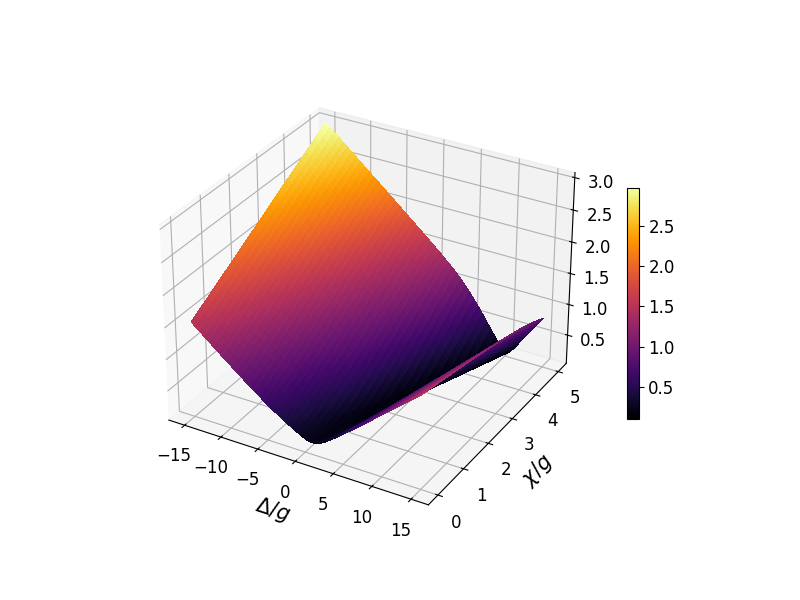
\includegraphics[width=\textwidth]{figuras/ch4/omega31 k=0.png}
%         \caption{}
%         \label{fig4:rabi chi}
%     \end{subfigure}
%     \vfill
%     \begin{subfigure}{0.3\textwidth}
%         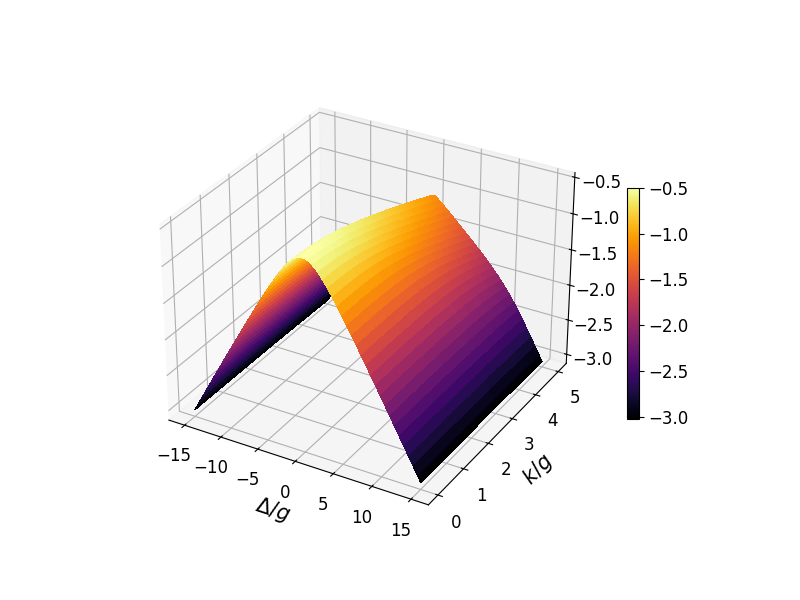
\includegraphics[width=\textwidth]{figuras/ch4/omega12 x=0.png}
%         \caption{}
%         \label{fig4:rabi chi}
%     \end{subfigure}
%     \hfill
%     \begin{subfigure}{0.3\textwidth}
%         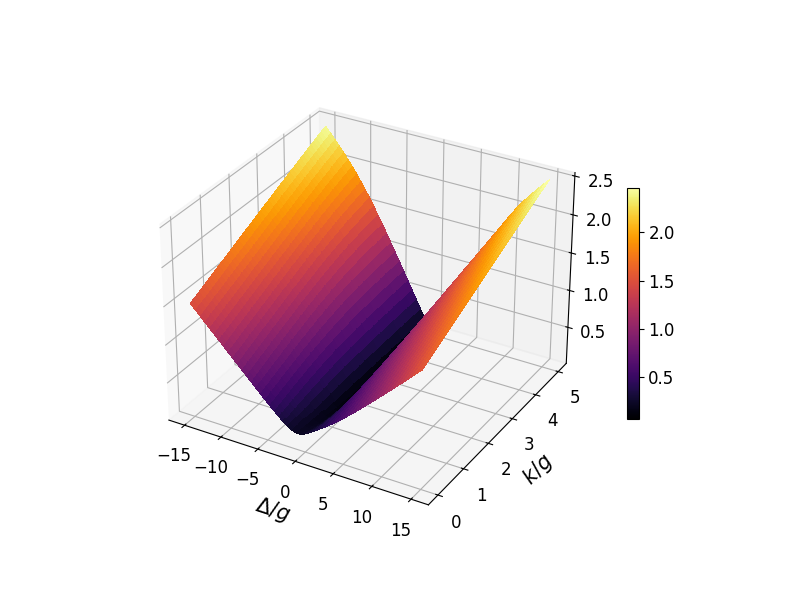
\includegraphics[width=\textwidth]{figuras/ch4/omega23 x=0.png}
%         \caption{}
%         \label{fig4:rabi chi}
%     \end{subfigure}
%     \hfill
%     \begin{subfigure}{0.3\textwidth}
%         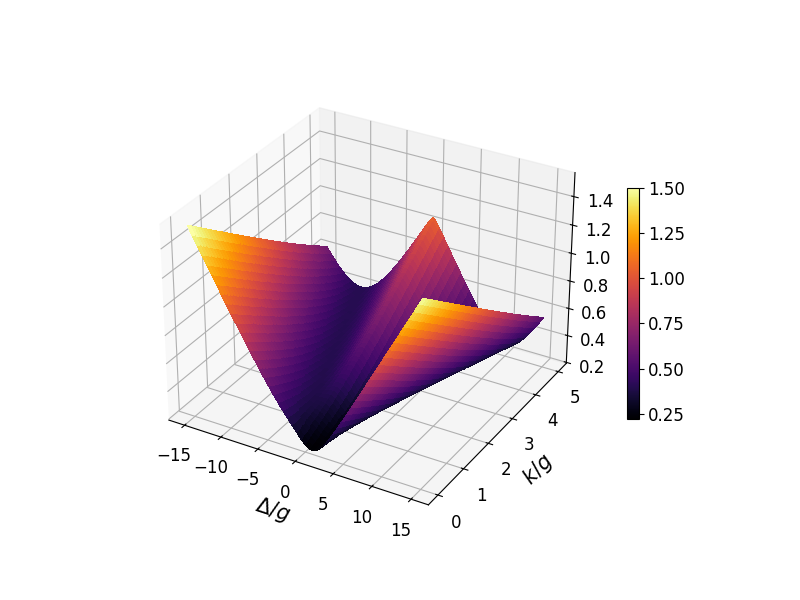
\includegraphics[width=\textwidth]{figuras/ch4/omega31 x=0.png}
%         \caption{}
%         \label{fig4:rabi chi}
%     \end{subfigure}
%     \caption{Frecuencias de Rabi en función del detunning, para diferentes valores de $\chi/g\in[0,5]$ y $k-J=0.5g$. A la izquierda $\Omega_{12}$ y a la derecha $\Omega_{23}$ y $\Omega_{13}$}
%     \label{}
% \end{figure}

Al cambiar las no linealidades del medio $\chi$ (Figura \ref{fig4:rabi 1 chi} y \ref{sub@fig4:rabi 2 chi}), la frecuencia $\Omega^{(2)}_{12}$ se comporta de manera similar a la frecuencia de Rabi del JC de 1 átomo, que es también igual a la $\Omega^{(1)}$. En ambos casos la diferencia de energía tiene un máximo que se desplaza lateralmente al aumentar el parámetro $\chi\in[0,5g]$, pero presenta una sutil diferencia, ya que también el máximo aumenta en valor absoluto. En la figura \ref{fig4:rabi 1 k} y \ref{sub@fig4:rabi 2 k} se explora el efecto de modificar $k-J\in [0,5g]$, donde el máximo ya no se desplaza lateralmente, sino que aumenta en valor absoluto. Por otro lado, en los paneles derechos, se puede analizar qué sucede con las frecuencias $\Omega^{(2)}_{23}$ y $\Omega^{(2)}_{31}$ al aumentar $\chi$ (Fig. \ref{fig4:rabi 2 chi}) y $k-J$ (Fig. \ref{fig4:rabi 2 k}). Es interesante notar como al aumentar $\chi$, se comienza a observar un máximo y mínimo local para la frecuencia $\Omega^{(2)}_{23}$ (rama superior). Similarmente, pero en la rama inferior, se observa este mismo comportamiento al aumentar $k-J$.


La dinámica para el caso de $N\geq2$ es muy complicada, ya que ahora se tienen 3 frecuencias diferentes, y predecir que sucede para cada combinación de parámetros y para cada condición inicial se hace muy complicado, por lo tanto, el análisis para estos casos no puede ser muy profundo. Lo que se puede distinguir es que cuando $\chi,k-J>g$, se comienzan a observar estos mínimos y máximos locales en las frecuencias, y se puede estudiar cuál es el efecto que tiene esto en el entrelazamiento de los átomos, y también si hay alguna relación entre los parámetros, por ejemplo como se encontró para el caso de 1 átomo (y para el subespacio de N=1) que hay una clara relación entre el detunning $\Delta$ y el medio $\chi$. En particular, es de interés encontrar una condición de robustez, similar a la Ec. (\ref{ec3:condicion robuestez 1 atomo}).

\section{Dinámica de entrelazamiento}
Para estudiar la dinámica de entrelazamiento entre los dos átomos $\rho_{AB}=\tr_C\{\rho\}$, se utilizará la concurrencia medida de entrelazamiento definida por la Ec. (\ref{ec4:concurrencia}) ($0\leq C_{AB} \leq 1$).

Lo primero que se analiza son los efectos de las interacciones entre los átomos. Se diferencian dos regímenes, el de Strong Interacting (SI) y Weak Interacting (WI), refiriéndose a la interacción entre los átomos con respecto a la cavidad. El SI será cuando la interacción entre los átomos es fuerte en comparación con la cavidad, es decir $k-J>g$, y WI con $k,J<g$. Ya que no se encontró un limite muy claro, se utilizará un valor representativo de cada régimen, $k-J=0.5g$ y $k-J=2.5g$ respectivamente, además de utilizar un parámetro del entorno $\gamma=0.25g$. Para ilustrar las diferencias entre condiciones iniciales, y para seguir con el paralelismo con el caso de 1 átomo, se considerarán únicamente las siguientes condiciones iniciales:
\begin{itemize}
    \item $\ket{eg0+ge0}$ para seguir el paralelismo con el JCM de 1 átomo 
    \item $\ket{eg1+ge1}$ para comparar con el anterior y explorar el subespacio $N=2$.
    %\item $\ket{ee0+gg2}$ para ver otra condición inicial con $N=2$ en donde los átomos \textbf{no} están entrelazados
\end{itemize}

Para comparar el efecto de los parámetros entre sí, todos los gráficos que se muestran en el resto del capítulo estarán caracterizados por un acoplamiento con el entorno de $\gamma=0.25g$, y todos los tiempos estarán normalizados según un periodo $T_0=2\pi/\Omega_0 \, | \Omega_0=\Omega^{(1)}(\Delta=0,\chi=0,k-J=0)$.
\subsection{Dependencia con el detunning}
\subsubsection{\underline{Condición inicial $\ket{eg0+ge0}$}}
\begin{figure}[h]
    \centering
    \begin{subfigure}{0.49\textwidth}
        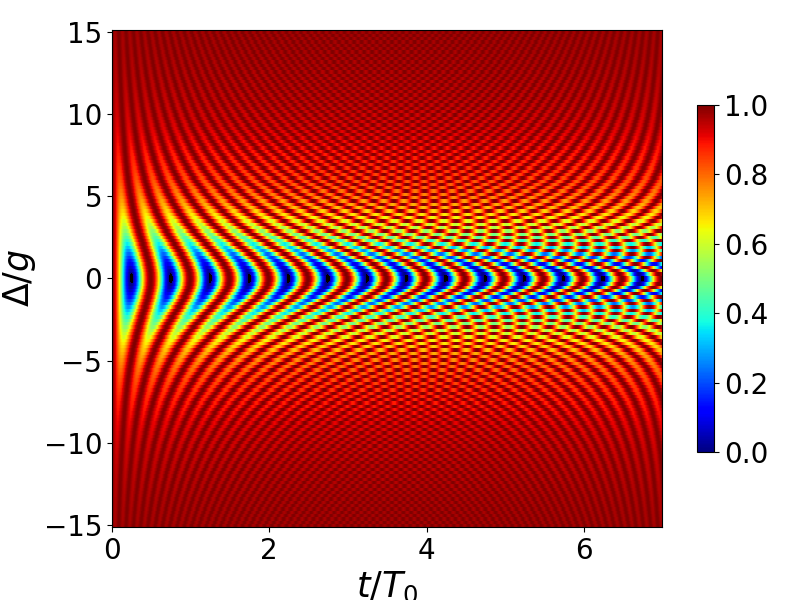
\includegraphics[width=\textwidth]{figuras/ch4/concu/delta/eg0+ge0 k=0.0g x=0.0g J=0.0g gamma=0.25g concu delta uni.png}
        \caption{}
        \label{fig4:concu detunning 0 uni}
    \end{subfigure}
    \hfill
    \begin{subfigure}{0.49\textwidth}
        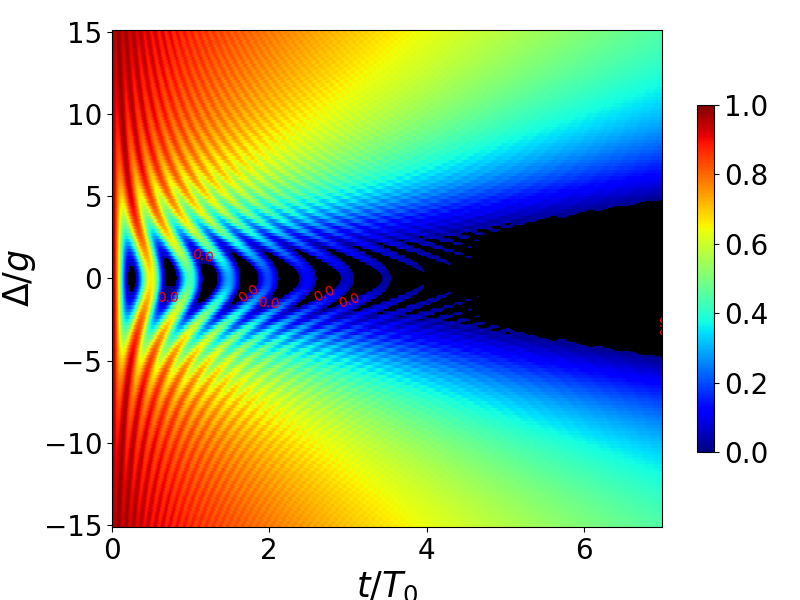
\includegraphics[width=\textwidth]{figuras/ch4/concu/delta/eg0+ge0 k=0.0g x=0.0g J=0.0g gamma=0.25g concu delta dis.png}
        \caption{}
        \label{fig4:concu detunning 0 dis}
    \end{subfigure}
    \caption{Dinámica de entrelazamiento para el estado inicial $\ket{eg0+ge0}$, en función del detunning, y para $\chi=k-J=0$.(a) Dinámica sin pérdidas,(b) Dinámica con pérdidas}
    \label{fig4:concu detunning 0}
\end{figure}
En la figura \ref{fig4:concu detunning 0} se observa la evolución de la concurrencia para la condición inicial $\ket{eg0+ge0}$, cuyo entrelazamiento entre los átomos es máximo. El eje x es el tiempo, y el eje y es el detunning $\Delta/g$. En el panel \ref{fig4:concu detunning 0 uni} se muestra el caso sin pérdidas; lo primero que se aprecia es que la figura es simétrica sobre $\Delta=0$ (caso resonante), y las oscilaciones son de menor frecuencia pero de mayor amplitud. A medida que se aumenta el valor absoluto del detunning, entonces las oscilaciones son de mayor frecuencia y menor amplitud. Consecuentemente, al tomar la dinámica disipativa, en el panel (\ref{sub@fig4:concu detunning 0 dis}), las oscilaciones siguen estando, pero ahora su máximo disminuye con el tiempo. Esto es de esperar, ya que la cavidad deja escapar fotones y el estado del sistema se hace mixto. Un estado mixto ya no es entrelazado, porque no hay coherencias, entonces se observa el deterioro del entrelazamiento a medida que el tiempo avanza. Hay otros dos comportamientos notables. 
Por un lado, se observa como el máximo del entrelazamiento decae más lentamente para valores más altos del detunning, esto se debe a la naturaleza de la dinámica poblacional; al aumentar el detunning, como se vio anteriormente, uno de los efectos principales es que las oscilaciones entre los estados tienen poca amplitud, y en este caso, esto implica que si bien el estado $\ket{gg1}$ tiene amplitud no nula, principalmente la probabilidad está concentrada en el estado inicial, que no sufre decoherencia por pérdida de fotones, ya que no tiene fotones en la cavidad. Entonces, mientras mayor el detunning, menor la probabilidad de encontrar al sistema en el estado $\ket{gg1}$, y por lo tanto tiene pocas probabilidades de perder fotones. Por otro lado, un efecto frecuente en este tipo de sistemas, es la muerte y reanimación súbita del entrelazamiento, que se nombran SDE (Sudden Death Effect) y SBE (Sudden Birth Effect) por sus siglas en inglés. En el caso disipativo, se marcaron zonas en negro, estas muestran como el entrelazamiento \textit{muere} durante un tiempo finito y revive luego. Este efecto es sorprendente, ya que se espera que las coherencias, responsables en gran medida del entrelazamiento entre átomos, decaigan asintóticamente. Este efecto muestra que esto no es así para algunos sistemas, y aún cuando las coherencias son distintas de cero, el entrelazamiento puede ser nulo durante un tiempo, y luego reaparecer súbitamente. La razón por la que aparece este fenómeno es que se está tomando traza parcial sobre la cavidad, lo que hace que algunas coherencias desaparezcan. aún así, no se entiende bien el porque de este efecto \cite{Roncaglia2008}.

La pregunta natural que sigue es si cambiar los parámetros $\chi$ y $k-J$, cambian la forma de la figura \ref{fig4:concu detunning 0}. En la figura \ref{fig4:concu detunning 0 params} se muestra nuevamente la dinámica de entrelazamiento en función del detunning, donde se modificó alguno de los parámetros:

\begin{figure}[h]
    \centering
    \begin{subfigure}{0.49\textwidth}
        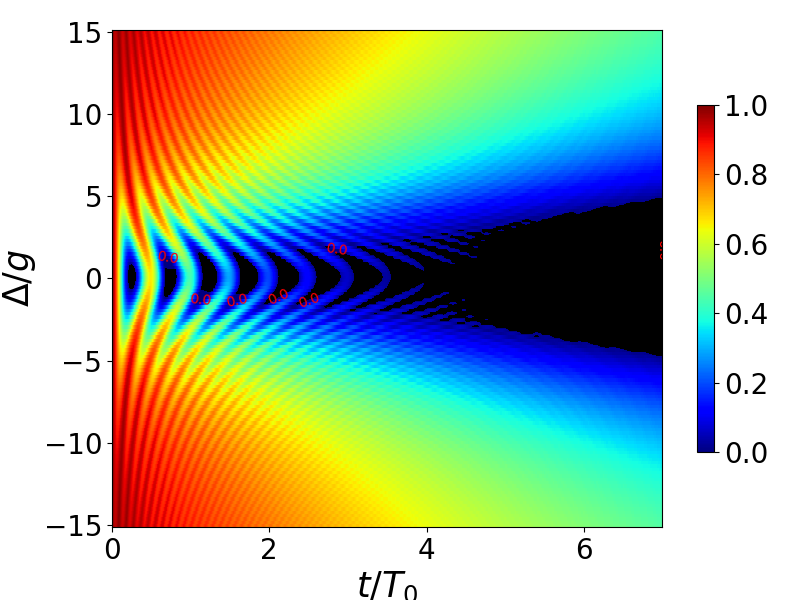
\includegraphics[width=\textwidth]{figuras/ch4/concu/delta/eg0+ge0 k=0.0g x=0.1g J=0.0g gamma=0.25g concu delta dis.png}
        \caption{$\chi=0.1g$}
        \label{fig4:concu detunning x1}
    \end{subfigure}
    \hfill
    \begin{subfigure}{0.49\textwidth}
        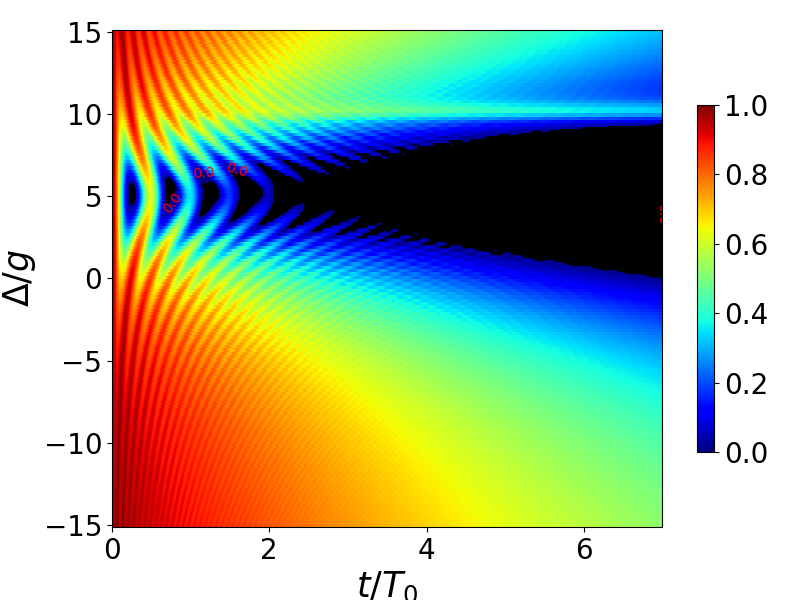
\includegraphics[width=\textwidth]{figuras/ch4/concu/delta/eg0+ge0 k=0.0g x=5.0g J=0.0g gamma=0.25g concu delta dis.png}
        \caption{$\chi=5g$}
        \label{fig4:concu detunning x2}
    \end{subfigure}
    \vfill
    \begin{subfigure}{0.49\textwidth}
        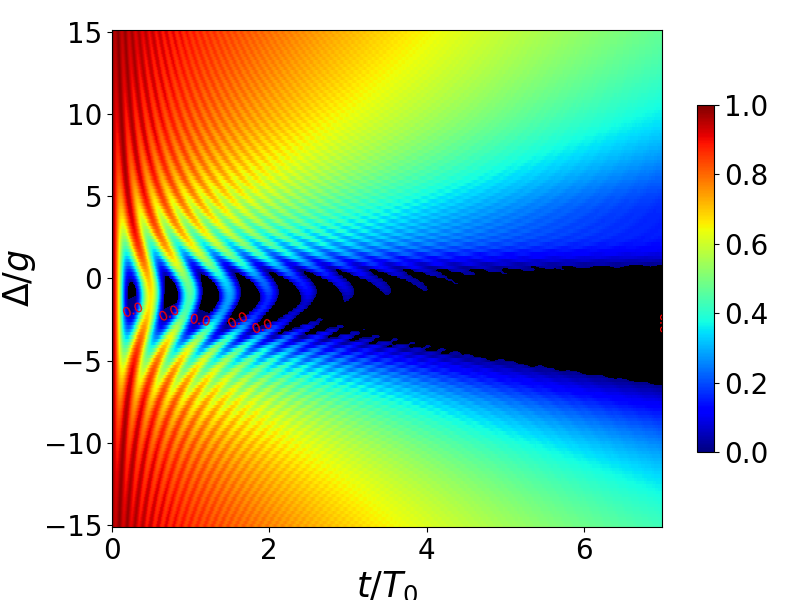
\includegraphics[width=\textwidth]{figuras/ch4/concu/delta/eg0+ge0 k=0.5g x=0.0g J=0.0g gamma=0.25g concu delta dis.png}
        \caption{$k-J=0.5g$}
        \label{fig4:concu detunning k1}
    \end{subfigure}
    \hfill
    \begin{subfigure}{0.49\textwidth}
        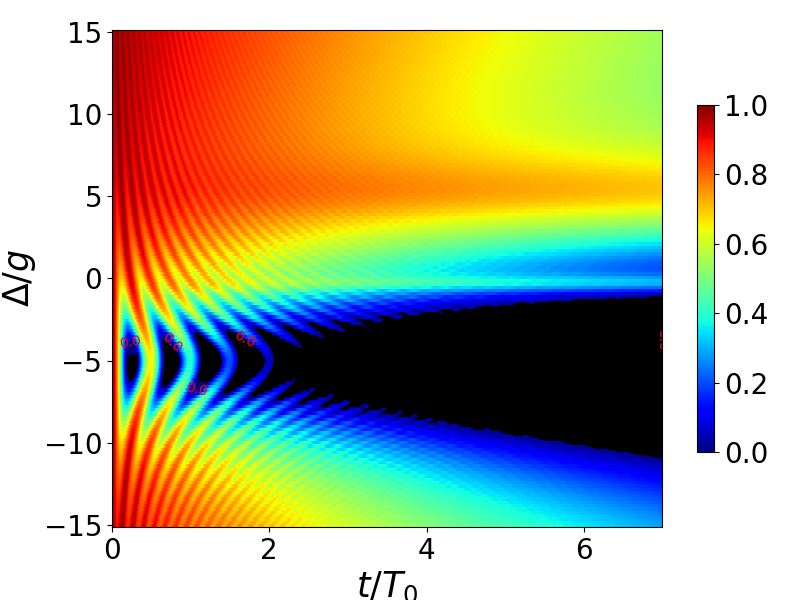
\includegraphics[width=\textwidth]{figuras/ch4/concu/delta/eg0+ge0 k=2.5g x=0.0g J=0.0g gamma=0.25g concu delta dis.png}
        \caption{$k-J=2.5g$}
        \label{fig4:concu detunning k2}
    \end{subfigure}
    \caption{Concurrencia en función del tiempo (eje x) y el detunning $\Delta$ (eje y) para el estado inicial $\ket{eg0+ge0}$, con diferentes parámetros (a) $\chi=0.1g$, $k-J=0$; (b) $\chi=5g$, $k-J=0$; (c) $\chi=0$, $k-J=0.5g$; (d) $\chi=0$, $k-J=2.5g$.}
    \label{fig4:concu detunning 0 params}
\end{figure}
En el las Figuras \ref{fig4:concu detunning x1} y \ref{fig4:concu detunning x2} se muestran dos casos en donde se puso de manifiesto la no linealidad del medio, cuyos parámetros son $\chi=0.1g$ y $\chi=5g$ respectivamente, ambos casos en presencia del entorno. Al comparar con la figura \ref{fig4:concu detunning 0 dis}, la forma cambia al aumentar las no linealidades, y la figura ya no es simétrica. De todas formas, cerca del centro ($\Delta/g=5$) el comportamiento es similar, y por lo tanto podría esperarse que este eje será el caso coherente, que en analogía con la sección \ref{sec3:fg disipacion}, puede ser una posible condición de robustez para la fase geométrica. Esto se analizará más tarde. En los paneles \ref{fig4:concu detunning k1} y \ref{fig4:concu detunning k2} se muestra el cambio al considerar acoplamiento entre los átomos, dados por una intensidad de $k-J=0.5g$ y $k-J=2.5g$ respectivamente. Nuevamente hay un desplazamiento, que se comporta igual que en el caso anterior, pero ahora el desplazamiento del eje es el doble que el aumento del parámetro de estudio, por ejemplo, si $k-J=2.5g$, entonces la figura se desplaza y su \textit{centro} está en $\Delta_0=-2(k-J)=-5g$. Esto no es tan sorprendente si se observa la expresión de la energía Ec. (\ref{ec4:energias n1}), donde los parámetros $\chi$ y $\Delta$ aparecen con un factor $1/2$, mientras que $k-J$ no. 

La simetría de la figura se rompe en una dirección, y se ve como hay, en ambos casos, una franja donde el entrelazamiento parece mantenerse durante un periodo más largo de tiempo. Además, se observa como en el panel \ref{fig4:concu detunning k2} que se corresponde con el caso $k-J=2.5g$, en la parte superior de la imagen, el entrelazamiento persiste mayor tiempo que su contraparte de menor interacción (panel \ref{fig4:concu detunning k1}) con $k-J=0.5g$.

Básicamente, el subespacio de $N=1$ se comporta igual que el Jaynes-Cummings de 1 átomo, pero donde se tiene un estado \textit{inerte}, el estado $\ket{eg0-ge0}$ que no interactúa con los otros dos. Esto puede servir para, usando como condición inicial el estado $\ket{\psi_0}=\cos\theta\ket{eg0}+\sin\theta\ket{ge0}$ que es combinación lineal de los estados $\ket{eg0\pm ge0}$, donde el estado simétrico evoluciona como siempre, y el antisimétrico no evoluciona, teniendo así una manera de mantener el entrelazamiento siempre por arriba de un cierto valor, que depende del valor de $\theta$, aún en presencia de decoherencia, ya que el estado $\ket{eg0-ge0}$ es un estado que no sufre pérdidas.

Por otro lado, cuando $\Delta-\chi+$
\subsubsection{\underline{Condición inicial $\ket{eg1+ge1}$}}
Ahora se estudia la dinámica para el estado simétrico en el subespacio de $N=2$. Igual que en el caso anterior, la figura \ref{fig4:concu detunning 1} muestra la evolución unitaria a la izquierda, y la disipativa a la derecha. En este subespacio hay más estructura, y si bien sigue siendo simétrico con respecto al eje $\Delta=0$, la forma es más complicada, y en el caso unitario también se observan regiones que presentan SDE, cosa que para $N=1$ no. Al igual que antes, al aumentar el detunning las oscilaciones son de mayor frecuencia y menor amplitud, conservando mejor el entrelazamiento. La razón es la misma: si bien ahora el estado $\ket{eg1+ge1}$ si puede perder fotones, al hacerlo cae al estado $\ket{eg0+ge0}$, que tiene el mismo entrelazamiento, y los otros dos estados del subespacio $\ket{gg2}$ decae al $\ket{gg1}$, y $\ket{ee0}$ no tiene fotones así que no pierde excitaciones. Por lo tanto, en el caso de alta desintonía, el comportamiento es similar al de anterior: las oscilaciones no tienen mucha amplitud y por lo tanto la probabilidad está concentrada casi toda en el estado $\ket{eg1+ge1}$, que al perder un fotón decae al estado $\ket{eg0+ge0}$ cuyo entrelazamiento es el mismo.
\begin{figure}[H]
    \centering
    \begin{subfigure}{0.49\textwidth}
        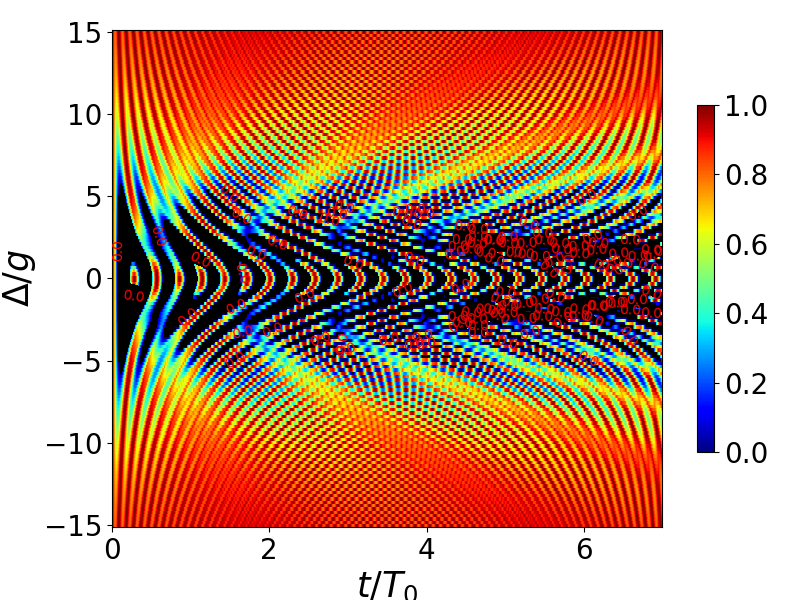
\includegraphics[width=\textwidth]{figuras/ch4/concu/delta/eg1+ge1 k=0.0g x=0.0g J=0.0g gamma=0.25g concu delta uni.png}
        \caption{}
        \label{fig4:concu detunning 1 uni}
    \end{subfigure}
    \hfill
    \begin{subfigure}{0.49\textwidth}
        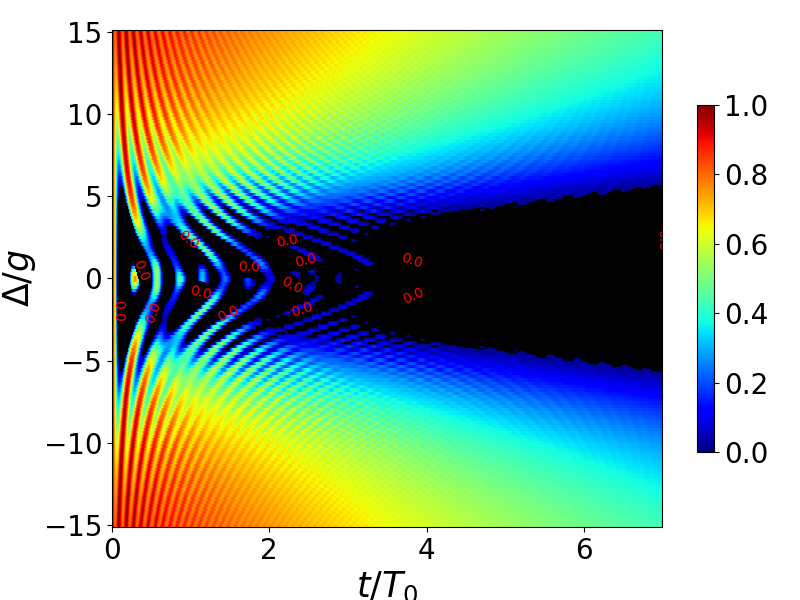
\includegraphics[width=\textwidth]{figuras/ch4/concu/delta/eg1+ge1 k=0.0g x=0.0g J=0.0g gamma=0.25g concu delta dis.png}
        \caption{}
        \label{fig4:concu detunning 1 dis}
    \end{subfigure}
    \caption{Dinámica de entrelazamiento para el estado inicial $\ket{eg0+ge0}$, en función del detunning, y para $\chi=k-J=0$. (a) Dinámica sin pérdidas, (b) Dinámica con pérdidas.}
    \label{fig4:concu detunning 1}
\end{figure}

Este subespacio de mayor excitación es relevante, ya que las energías de los estados presentan máximos y mínimos locales en función de los parámetros del problema (figuras \ref{fig4:frecuencias de rabi}), lo que cambiara drásticamente el entrelazamiento al modificar los valores de los parámetros.
\begin{figure}[h]
    \centering
    \begin{subfigure}{0.49\textwidth}
        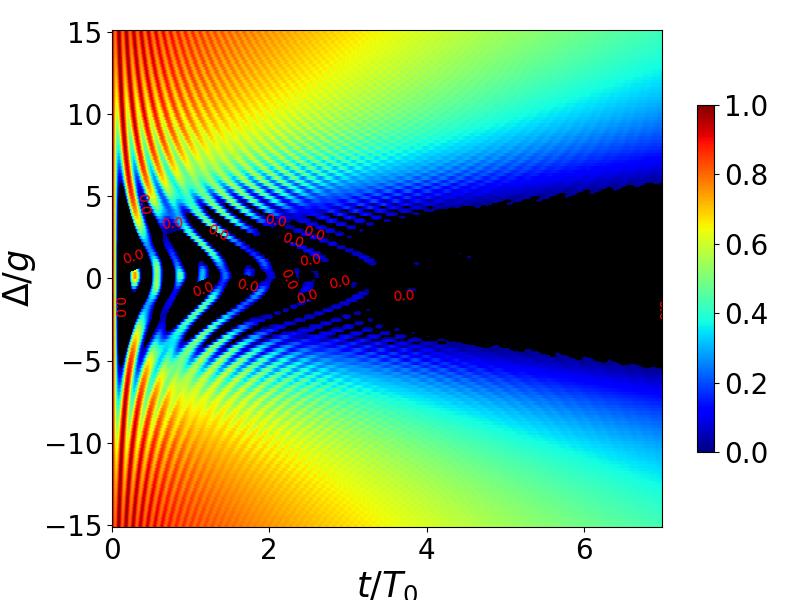
\includegraphics[width=\textwidth]{figuras/ch4/concu/delta/eg1+ge1 k=0.0g x=0.1g J=0.0g gamma=0.25g concu delta dis.png}
        \caption{$\chi=0.1g$}
        \label{fig4:concu detunning 1 x1}
    \end{subfigure}
    \hfill
    \begin{subfigure}{0.49\textwidth}
        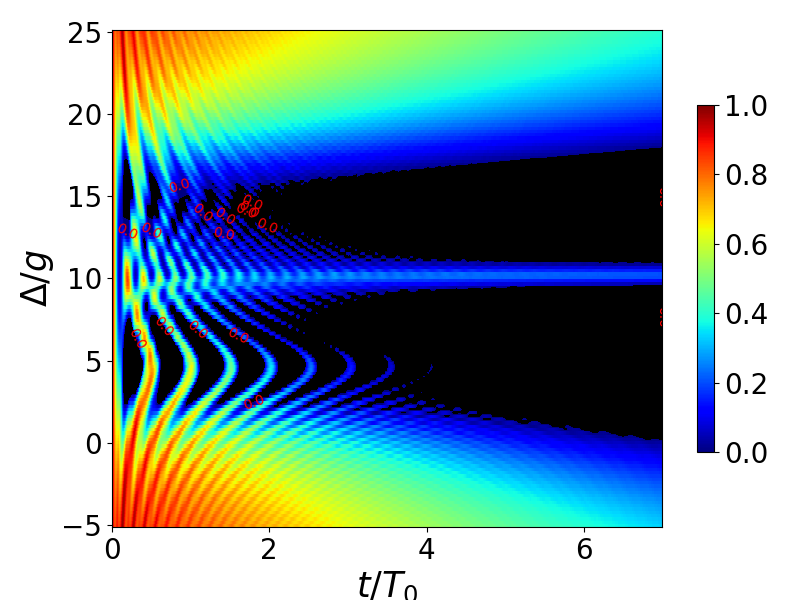
\includegraphics[width=\textwidth]{figuras/ch4/concu/delta/eg1+ge1 k=0.0g x=5.0g J=0.0g gamma=0.25g concu delta dis.png}
        \caption{$\chi=5g$}
        \label{fig4:concu detunning 1 x2}
    \end{subfigure}
    \vfill
    \begin{subfigure}{0.49\textwidth}
        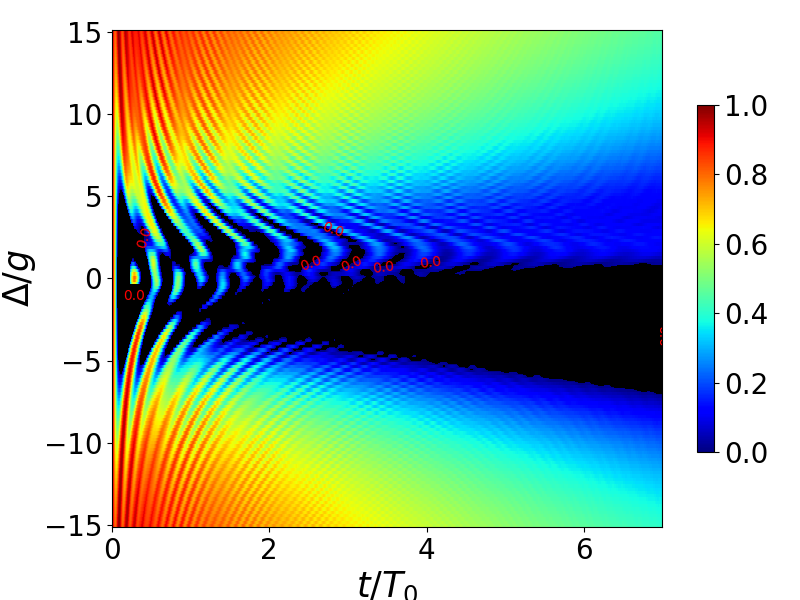
\includegraphics[width=\textwidth]{figuras/ch4/concu/delta/eg1+ge1 k=0.5g x=0.0g J=0.0g gamma=0.25g concu delta dis.png}
        \caption{$k-J=0.5g$}
        \label{fig4:concu detunning 1 k1}
    \end{subfigure}
    \hfill
    \begin{subfigure}{0.49\textwidth}
        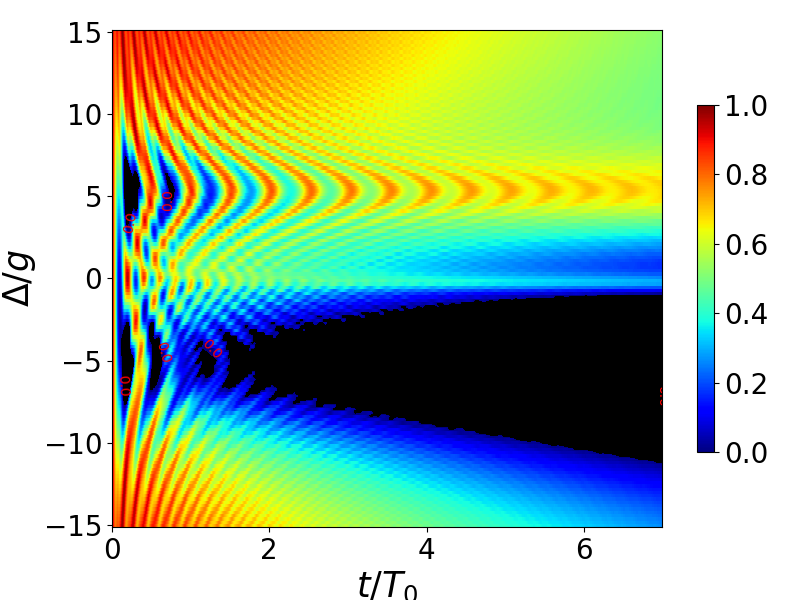
\includegraphics[width=\textwidth]{figuras/ch4/concu/delta/eg1+ge1 k=2.5g x=0.0g J=0.0g gamma=0.25g concu delta dis.png}
        \caption{$k-J=2.5g$}
        \label{fig4:concu detunning 1 k2}
    \end{subfigure}
    \caption{Dinámica de entrelazamiento para $\ket{eg1+ge1}$ en función del detunning, variando parámetros. (\ref{sub@fig4:concu detunning x1}) $\chi=0.1g$, $k-J=0$; (\ref{sub@fig4:concu detunning x2}) $\chi=5g$, $k-J=0$; (\ref{sub@fig4:concu detunning k1}) $\chi=0$, $k-J=0.5g$; (\ref{sub@fig4:concu detunning k2}) $\chi=0$, $k-J=2.5g$ }
    \label{fig4:concu detunning 1 params}
\end{figure}
En la figura \ref{fig4:concu detunning 1 params} se muestran diferentes casos. En la primera fila los casos con medio Kerr cuyos parámetros son $\chi=0.1g$ y $\chi=5g$ respectivamente. En la figura \ref{fig4:concu detunning x1} correspondiente a $\chi=0.1g$, no se observa ningún cambio significativo con respecto al caso $\chi=0$, es muy pequeño para ser notado y la estructura queda igual. Pero al aumentar mucho la no linealidad del medio, se comienza a observar el desdoblamiento en las energías, y los máximos y mínimos locales comienzan a tomar importancia. En la figura \ref{fig4:concu detunning 1 x2} se ve como hay dos zonas en donde las oscilaciones tienen gran amplitud y poca frecuencia, similar al caso \textit{resonante}. Esto se puede explicar con el desdoblamiento de energías. Hay dos mínimos en las frecuencias de Rabi que participan en este proceso, que están ceca de en $\Delta_1=5g$ y $\Delta_2=15g$ aproximadamente. Haciendo una analogía con el caso de 1 átomo, donde se vio que la condición de robustez se daba para $\Delta=\chi(2n_c-1)$ (ver (\ref{sec3:medio kerr})) y recordando que esta condición se obtiene de la diferencia entre las contribuciones diagonales del Hamiltoniano, entonces en este caso, se puede hacer lo mismo y obtener dos condiciones, la primera con $\chi n_c^2-\chi(n_c-1)^2=\chi(2n_c-1)$ que es igual a la del caso de $N=1$, y la segunda con $\chi(n_c-1)^2-\chi(n_c-2)^2=\chi(2n_c-3)$. Sustituyendo $n=2$, la condición se da para $\Delta=\chi$ y $\Delta=3\chi$, que es justo donde se aprecian los mínimos. Si bien el segundo mínimo de $3\chi$ parece ser menos pronunciado, esta analogía funciona bien.

Si se hace esta resta pero ahora con $\chi=0$ y nos concentramos en $k-J$, la condición se da cuando $\Delta=\pm 2(k-J)$, que es donde se observan los mínimos del entrelazamiento en la figura \ref{fig4:concu detunning 1 k2}. En general entonces, se puede decir que esta condición de menor frecuencia y mayor amplitud de oscilación se da cuando las energías de los estados están cerca de la degeneración, y como hay 3 estados que interactúan siempre por medio del estado del medio (el $\ket{egn+gen}$), entonces puede tres casos de degeneración, que se dan en el caso general cuando

\begin{equation}
    \Delta-\chi(2n-1)+2(k-J)=0,
    \label{ec4:condicion 1}
\end{equation}
que se corresponde con la degeneración entre las energías del estado $\ket{ggn}$ y $(\ket{eg,n-1}+\ket{ge,n-1})/\sqrt{2}$, y en el otro caso
\begin{equation}
    \Delta-\chi(2n-3)-2(k-J)=0,
    \label{ec4:condicion 2}
\end{equation}
que se corresponde con los estados $(\ket{eg,n-1}+\ket{ge,n-1})/\sqrt{2}$ y $\ket{ee,n-2}$. También, se puede dar que los tres estados están degenerados si se cumplen las dos condiciones simultáneamente.
\textcolor{orange}{
La tercera condición que se puede dar es cuando los estados $\ket{ggn}$ y $\ket{ee,n-2}$ son degenerados. Si bien estos no interactúan directamente entre si, el estado $\ket{eg1+ge1}$ interactúa con ambos, y si estos son degenerados, entonces están en igualdad de condiciones ante el estado inicial. Por lo tanto, la ultima condición se da cuando
\begin{equation}
    \Delta-2\chi(n-1)=0.
    \label{ec4:condicion 3}
\end{equation}
En particular para $n=2$ se tiene que $\Delta=2\chi$. En las figuras \ref{fig4:concu detunning 1 x2} y \ref{fig4:concu detunning 1 k2}, se observa que cuando se cumple esta condición, el entrelazamiento es más fuerte ante el efecto del entorno.  
}
%\subsubsection{\underline{Condición inicial $\ket{ee0+gg2}$}}
%Esta condición inicial no tiene entrelazamiento inicial, ya que al tomar traza parcial sobre la cavidad, uno de los estados de la superposición tiene 0 fotones, y el otro 2, entonces el resultado de trazar sobre la cavidad en el instante inicial es que los átomos se encuentren en el estado máximamente mixto $\frac{1}{2}(\ketbra{ee}{ee}+\ketbra{gg}{gg})$, que no es entrelazado.

\subsection{Dependencia con el medio $\chi$}
\subsubsection{\underline{Condición inicial $\ket{eg0+ge0}$}}
En la figura \ref{fig4:concu x 0} se muestra la dinámica de entrelazamiento en función de la no linealidad del medio. No hay diferencias mayores con la dependencia en $\Delta$ (Figura \ref{fig4:concu detunning 0}).
\begin{figure}[h!]
    \centering
    \begin{subfigure}{0.49\textwidth}
        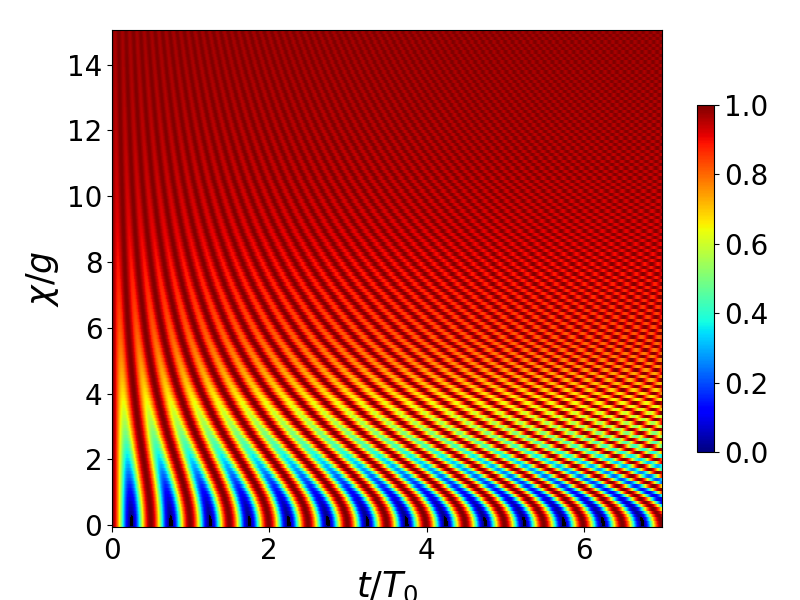
\includegraphics[width=\textwidth]{figuras/ch4/concu/chi/eg0+ge0 d=0.0g k=0.0g J=0.0g gamma=0.25g concu chi uni.png}
        \caption{}
        \label{fig4:concu x 0 uni}
    \end{subfigure}
    \hfill
    \begin{subfigure}{0.49\textwidth}
        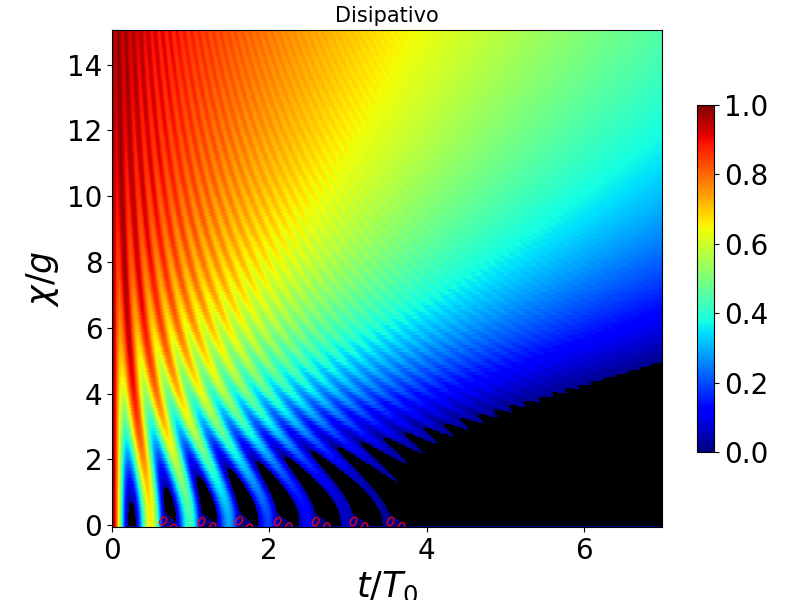
\includegraphics[width=\textwidth]{figuras/ch4/concu/chi/eg0+ge0 d=0.0g k=0.0g J=0.0g gamma=0.25g concu chi dis.png}
        \caption{}
        \label{fig4:concu x 0 dis}
    \end{subfigure}
    \caption{Dinámica de entrelazamiento para el estado inicial $\ket{eg0+ge0}$, en función del detunning, y para $\chi=k-J=0$.(a) Dinámica sin pérdidas,(b) Dinámica con pérdidas.}
    \label{fig4:concu x 0}
\end{figure}

Esto reafirma que en el espacio de $N=1$, el medio Kerr es muy similar al detunning. 

\begin{figure}[h!]
    \centering
    \begin{subfigure}{0.49\textwidth}
        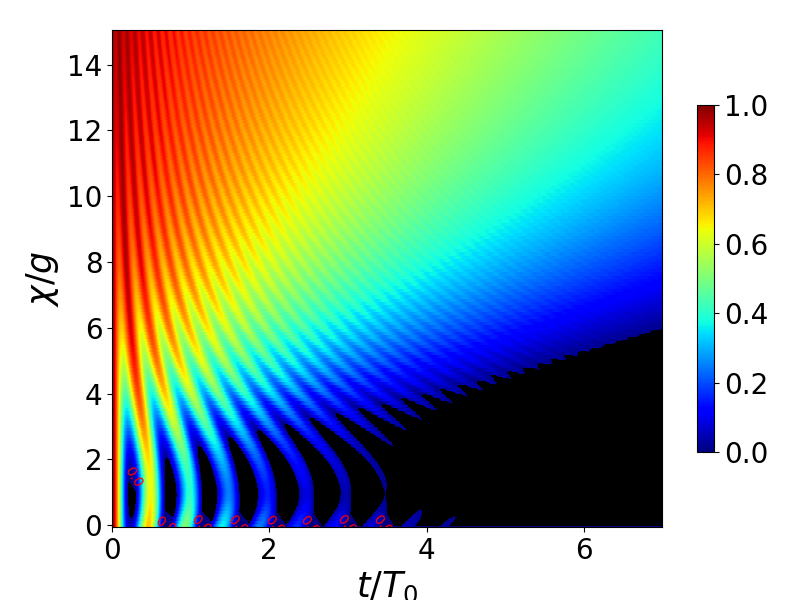
\includegraphics[width=\textwidth]{figuras/ch4/concu/chi/eg0+ge0 d=1.0g k=0.0g J=0.0g gamma=0.25g concu chi dis.png}
        \caption{$\Delta=1g$}
        \label{fig4:concu x d1}
    \end{subfigure}
    \hfill
    \begin{subfigure}{0.49\textwidth}
        \includegraphics[width=\textwidth]{figuras/ch4/concu/chi/eg0+ge0 d=5.0g k=0.0g J=0.0g gamma=0.25g concu chi dis.png}
        \caption{$\Delta=5g$}
        \label{fig4:concu x d2}
    \end{subfigure}
    \vfill
    \begin{subfigure}{0.49\textwidth}
        \includegraphics[width=\textwidth]{figuras/ch4/concu/chi/eg0+ge0 d=0.0g k=0.5g J=0.0g gamma=0.25g concu chi dis.png}
        \caption{$k-J=0.5g$}
        \label{fig4:concu x k1}
    \end{subfigure}
    \hfill
    \begin{subfigure}{0.49\textwidth}
        \includegraphics[width=\textwidth]{figuras/ch4/concu/chi/eg0+ge0 d=0.0g k=2.5g J=0.0g gamma=0.25g concu chi dis.png}
        \caption{$k-J=2.5g$}
        \label{fig4:concu x k2}
    \end{subfigure}
    \caption{Dinámica de entrelazamiento para condición inicial $\ket{eg0+ge0}$ en función del medio Kerr, para diferentes parámetros: (a) $\Delta=g$, $k-J=0$; (b) $\Delta=5g$, $k-J=0$; (c) $\Delta=0$, $k-J=0.5g$; (d) $\Delta=0$, $k-J=2.5g$.}
    \label{fig4:concu x params}
\end{figure}
\newpage
\subsubsection{\underline{Condición inicial $\ket{eg1+ge1}$}}
Para la condición inicial $\ket{eg1+ge1}$ en función de $\chi$ se observan diferencias con el caso del detunning: las imágenes \ref{fig4:concu x 1} y \ref{fig4:concu detunning 1} tienen diferentes estructuras. Esto significa que ya no están en igualdad de condiciones el detunning y el medio, como era el caso de el subespacio de $N=1$.
\begin{figure}[h!]
    \centering
    \begin{subfigure}{0.49\textwidth}
        \includegraphics[width=\textwidth]{figuras/ch4/concu/chi/eg1+ge1 d=0.0g k=0.0g J=0.0g gamma=0.25g concu chi uni.png}
        \caption{}
        \label{fig4:concu x 1 uni}
    \end{subfigure}
    \hfill
    \begin{subfigure}{0.49\textwidth}
        \includegraphics[width=\textwidth]{figuras/ch4/concu/chi/eg1+ge1 d=0.0g k=0.0g J=0.0g gamma=0.25g concu chi dis.png}
        \caption{}
        \label{fig4:concu x 1 dis}
    \end{subfigure}
    \caption{Dinámica de entrelazamiento para el estado inicial $\ket{eg1+ge1}$, en función del medio Kerr, y para $\Delta=k-J=0$. (a) Dinámica sin pérdidas,(b) Dinámica con pérdidas}
    \label{fig4:concu x 1}
\end{figure}
Aparte de esto, los demás comportamientos no son inesperados. Al aumentar $\chi$, el entrelazamiento inicial se conserva ya que las oscilaciones son de menor amplitud; ademas, al agregar disipación, las oscilaciones decaen en amplitud y las zonas donde hay presente SDE se agrandan. También, al aumentar la no linealidad del medio, la frecuencia de oscilación aumenta haciendo que el entrelazamiento sea más robusto ante el efecto del entorno.
\begin{figure}[h!]
    \centering
    \begin{subfigure}{0.49\textwidth}
        \includegraphics[width=\textwidth]{figuras/ch4/concu/chi/eg1+ge1 d=1.0g k=0.0g J=0.0g gamma=0.25g concu chi dis.png}
        \caption{$\Delta=1g$}
        \label{fig4:concu x 1 d1}
    \end{subfigure}
    \hfill
    \begin{subfigure}{0.49\textwidth}
        \includegraphics[width=\textwidth]{figuras/ch4/concu/chi/eg1+ge1 d=5.0g k=0.0g J=0.0g gamma=0.25g concu chi dis.png}
        \caption{$\Delta=5g$}
        \label{fig4:concu x 1 d2}
    \end{subfigure}
    \vfill
    \begin{subfigure}{0.49\textwidth}
        \includegraphics[width=\textwidth]{figuras/ch4/concu/chi/eg1+ge1 d=0.0g k=0.5g J=0.0g gamma=0.25g concu chi dis.png}
        \caption{$k-J=0.5g$}
        \label{fig4:concu x 1 k1}
    \end{subfigure}
    \hfill
    \begin{subfigure}{0.49\textwidth}
        \includegraphics[width=\textwidth]{figuras/ch4/concu/chi/eg1+ge1 d=0.0g k=2.5g J=0.0g gamma=0.25g concu chi dis.png}
        \caption{$k-J=2.5g$}
        \label{fig4:concu x 1 k2}
    \end{subfigure}
    \caption{Dinámica de entrelazamiento para $\ket{eg1+ge1}$ en función del medio Kerr, para diferentes valores: (a) $\Delta=g$, $k-J=0$; (b) $\Delta=5g$, $k-J=0$; (c) $\Delta=0$, $k-J=0.5g$; (d) $\Delta=0$, $k-J=2.5g$.}
    \label{fig4:concu x params 1}
\end{figure}
Al cambiar algunos de los parámetros para ver como afectan el entrelazamiento en función de $\chi$, se muestran en las figuras \ref{fig4:concu x 1 d1} y \ref{fig4:concu x 1 d2} como afecta aumentar el detunning. En primer lugar, aumentar a $\Delta=g$ no afecta sustancialmente la estructura (comparar con \ref{fig4:concu x 1 dis}), el efecto principal es desplazar hacia arriba la figura. Pero al aumentar mucho el detunning como en el caso de $\Delta=5g$, observamos que no solo que la frecuencia cambia (poco pero cambia, en el primer caso para llegar a $t/T_0=2$ se necesitan 3 oscilaciones pero para el segundo 4), como se esperaba, sino que también hay nuevamente una separación en dos regiones. Esto se atribuye a que la diferencia de energías tiene máximos y mínimos locales, haciendo que en estas regiones las oscilaciones sean de mayor amplitud. La estructura en las figuras \ref{fig4:concu x 1 k1} y \ref{sub@fig4:concu x 1 k2} cambian con respecto a las dos anteriores. Al aumentar la interacción entre los átomos, la zona de SDE se acentúa y ya no se aprecian oscilaciones que entran en la zona negra. Las diferencias principales son que para $\chi \approx 0$ en el caso de $k=J=2.5g$ parece conservar bien el entrelazamiento cosa que no es tan notable para el caso de $\Delta=5g$, y la segunda es que en la figura \ref{fig4:concu x 1 d2} cerca de $\chi=2.5g$ se observa también una franja que conserva mejor el entrelazamiento en comparación con los valores cercanos.
%\subsubsection{\underline{Condición inicial $\ket{ee0+gg2}$}}
\newpage
\subsection{Dependencia con la interacción entre átomos $k-J$}
Ahora nos concentraremos en la interacción entre los átomos. A diferencia de los otros dos parámetros, esta interacción solo depende los dos átomos y por lo tanto se esperan comportamientos diferentes. 
\subsubsection{\underline{Condición inicial $\ket{eg0+ge0}$}}
\begin{figure}[h!]
    \centering
    \begin{subfigure}{0.49\textwidth}
        \includegraphics[width=\textwidth]{figuras/ch4/concu/k/eg0+ge0 d=0.0g x=0.0g J=15.0g gamma=0.25g concu k uni.png}
        \caption{Dinámica sin pérdidas}
        \label{fig4:concu k 0 uni}
    \end{subfigure}
    \hfill
    \begin{subfigure}{0.49\textwidth}
        \includegraphics[width=\textwidth]{figuras/ch4/concu/k/eg0+ge0 d=0.0g x=0.0g J=15.0g gamma=0.25g concu k dis.png}
        \caption{Dinámica con pérdidas}
        \label{fig4:concu k 0 dis}
    \end{subfigure}
    \caption{Dinámica de entrelazamiento para el estado inicial $\ket{eg0+ge0}$, en función del detunning, y para $\chi=k-J=0$.}
    \label{fig4:concu k 0}
\end{figure}
Desde el comienzo ya se puede ver como al aumentar el valor absoluto de la interacción el comportamiento es el mismo que en los otros dos casos, donde aumenta la frecuencia y disminuye la amplitud conservando el entrelazamiento inicial, pero en es te caso este comportamiento se ve acentuado. 


\begin{figure}[h!]
    \centering
    \begin{subfigure}{0.49\textwidth}
        \includegraphics[width=\textwidth]{figuras/ch4/concu/k/eg0+ge0 d=1.0g x=0.0g J=15.0g gamma=0.25g concu k dis.png}
        \caption{$\Delta=1g$}
        \label{fig4:concu k d1}
    \end{subfigure}
    \hfill
    \begin{subfigure}{0.49\textwidth}
        \includegraphics[width=\textwidth]{figuras/ch4/concu/k/eg0+ge0 d=5.0g x=0.0g J=15.0g gamma=0.25g concu k dis.png}
        \caption{$\Delta=5g$}
        \label{fig4:concu k d2}
    \end{subfigure}
    \vfill
    \begin{subfigure}{0.49\textwidth}
        \includegraphics[width=\textwidth]{figuras/ch4/concu/k/eg0+ge0 d=0.0g x=0.5g J=15.0g gamma=0.25g concu k dis.png}
        \caption{$\chi=0.5g$}
        \label{fig4:concu k x1}
    \end{subfigure}
    \hfill
    \begin{subfigure}{0.49\textwidth}
        \includegraphics[width=\textwidth]{figuras/ch4/concu/k/eg0+ge0 d=0.0g x=5.0g J=15.0g gamma=0.25g concu k dis.png}
        \caption{$\chi=5g$}
        \label{fig4:concu k x2}
    \end{subfigure}
    \caption{Dinámica de entrelazamiento para condición inicial $\ket{eg0+ge0}$ variando: (a) $\Delta=g$, $\chi=0$; (b) $\Delta=5g$, $\chi=0$; (c) $\Delta=0$, $\chi=0.5g$; (d) $\Delta=0$, $\chi=5g$.}
    \label{fig4:concu k params}
\end{figure}

La interacción entre los átomos conserva mejor el entrelazamiento. Esto también se observa cuando se agrega la disipación, en comparación con las otras interacciones, en la figura \ref{fig4:concu k 0 uni} se ve como se conserva mejor el entrelazamiento.

En la figura \ref{fig4:concu k params} se observan los efectos que tienen los otros dos parámetros en la dinámica. Por un lado, vemos que aumentar el detunning \ref{fig4:concu k d1} desplaza el centro hacia abajo pero no parece haber mucha diferencia. Al seguir aumentando la desintonía \ref{fig4:concu k d2}, el centro se sigue desplazando y podemos ver que este se desplaza la mitad que lo que aumenta $\Delta$. Ademas, la estructura pierde la simetría y se observa una franja en la parte superior donde el entrelazamiento se conserva mejor. Este valor parece corresponderse con $+\Delta/2$. Esto puede deberse a la condición que se encontró anteriormente (\ref{ec4:condicion 1} y \ref{ec4:condicion 2}) que en este caso se resume en que la condición de degeneración se de para $k-J=\pm\Delta/2$. Es interesante que en este caso una de las condiciones presenta zonas de SDE, y la otra en cambio conserva mejor el entrelazamiento que las demás zonas. Por otro lado, al cambiar las no linealidades, vemos que el efecto es exactamente el mismo, pero el desplazamiento es ahora en el otro sentido, y las condiciones de degeneración siguen siendo las mismas, a menos de un signo.
\subsubsection{\underline{Condición inicial $\ket{eg1+ge1}$}}
Al considerar el espacio de $N=2$, lo primero que resalta es que la zona central que presenta SDE ahora es más ancha. Por otro lado, al agregar disipación, las diferencias parecen desaparecer con respecto a su contraparte de $N=1$. Esto probablemente se debe a que en presencia de disipación, para tiempos largos, el estado del sistema sera similar. Más aún considerando que se está ignorando la dinámica de la cavidad al observar el entrelazamiento entre los átomos.
\begin{figure}[h!]
    \centering
    \begin{subfigure}{0.49\textwidth}
        \includegraphics[width=\textwidth]{figuras/ch4/concu/k/eg1+ge1 d=0.0g x=0.0g J=15.0g gamma=0.25g concu k uni.png}
        \caption{}
        \label{fig4:concu k 1 uni}
    \end{subfigure}
    \hfill
    \begin{subfigure}{0.49\textwidth}
        \includegraphics[width=\textwidth]{figuras/ch4/concu/k/eg1+ge1 d=0.0g x=0.0g J=15.0g gamma=0.25g concu k dis.png}
        \caption{}
        \label{fig4:concu k 1 dis}
    \end{subfigure}
    \caption{Dinámica de entrelazamiento para el estado inicial $\ket{eg0+ge0}$, en función del detunning, y para $\chi=k-J=0$. (a) Dinámica sin pérdidas, (b) Dinámica con pérdidas}
    \label{fig4:concu k 1}
\end{figure}
La mayor diferencia entre ambos casos aparece cuando observamos los efectos de los parámetros $\Delta$ y $\chi$. Este caso es interesante porque nos ayuda a ver concretamente como, al tener ahora 3 estados dinámicos, el efecto del detunning y del medio son diferentes, que en el caso de 1 átomo (o en el subespacio de $N=1$) por lo que se vio antes son lo mismo. En la figura \ref{fig4:concu k params 1}\ref{sub@fig4:concu k 1 d2} y \ref{sub@fig4:concu k 1 x2} muestra la clara diferencia entre estos dos efectos. Para el detunning aparecen 2 regiones, que nuevamente son correctamente predichas por las condiciones \ref{ec4:condicion 1} y \ref{ec4:condicion 2} (considerando $\chi=0$), y para el caso del medio (panel \ref{sub@fig4:concu k 1 x2}) si traducimos las condiciones para $\Delta=0$ obtenemos que la condición de degeneración se da para $k-J=\frac{3}{2}\chi=7.5g$ y $k-J=\frac{-\chi}{2}=-2.5g$, que es justamente donde se observan las regiones con mayor estructura.
Esto nos dice que fundamentalmente, la degeneración de estados lleva a una mayor coherencia entre las oscilaciones del entrelazamiento. Si bien esto es cierto, puede ser que este entrelazamiento muera súbitamente, o que sea más robusto que otras combinaciones de parámetros. Esto se ve claramente en estas dos figuras (paneles \ref{sub@fig4:concu k 1 d2} y \ref{sub@fig4:concu k 1 x2}), donde se pudo predecir correctamente que había zonas más coherentes, pero en ambos casos tenemos una de las zonas que presenta SDE y el entrelazamiento muere, y la segunda zona donde las oscilaciones perduran en el tiempo más que en cualquier otra combinación de parámetros. 
\begin{figure}[h!]
    \centering
    \begin{subfigure}{0.49\textwidth}
        \includegraphics[width=\textwidth]{figuras/ch4/concu/k/eg1+ge1 d=1.0g x=0.0g J=15.0g gamma=0.25g concu k dis.png}
        \caption{$\Delta=1g$}
        \label{fig4:concu k 1 d1}
    \end{subfigure}
    \hfill
    \begin{subfigure}{0.49\textwidth}
        \includegraphics[width=\textwidth]{figuras/ch4/concu/k/eg1+ge1 d=5.0g x=0.0g J=15.0g gamma=0.25g concu k dis.png}
        \caption{$\Delta=5g$}
        \label{fig4:concu k 1 d2}
    \end{subfigure}
    \vfill
    \begin{subfigure}{0.49\textwidth}
        \includegraphics[width=\textwidth]{figuras/ch4/concu/k/eg1+ge1 d=0.0g x=0.5g J=15.0g gamma=0.25g concu k dis.png}
        \caption{$\chi=0.5g$}
        \label{fig4:concu k 1 x1}
    \end{subfigure}
    \hfill
    \begin{subfigure}{0.49\textwidth}
        \includegraphics[width=\textwidth]{figuras/ch4/concu/k/eg1+ge1 d=0.0g x=5.0g J=15.0g gamma=0.25g concu k dis.png}
        \caption{$\chi=5g$}
        \label{fig4:concu k 1 x2}
    \end{subfigure}
    \caption{Dinámica de entrelazamiento para condición inicial $\ket{eg1+ge1}$ variando: (a) $\Delta=g$, $\chi=0$; (b) $\Delta=5g$, $\chi=0$; (c) $\Delta=0$, $\chi=0.5g$; (d) $\Delta=0$, $\chi=5g$.}
    \label{fig4:concu k params 1}
\end{figure}
%\subsubsection{\underline{Condición inicial $\ket{3er0}$}}


\subsection{Acoplamiento Buck-Sukumar}
Se repitió el estudio utilizando el acoplamiento no lineal entre la cavidad y los átomos, este acoplamiento es mayor mientras más excitaciones tenga la cavidad, concretamente la intensidad del acoplamiento se multiplica por la raíz de la cantidad de fotones de la cavidad $\sqrt{n_C}$. 
La conclusión de este estudio es que en el caso de $N=1$, es todo exactamente igual. Para $N=2$, hay algunas pequeñas diferencias, pero son casi insignificantes y no tienen consecuencias mayores sobre el entrelazamiento de los átomos. 

Por lo tanto, no justifica mostrar nada, solo mencionar que en los casos observados no afecta significativamente.

\section{Conclusiones del capítulo 4}
En este capítulo se analizó la dinámica del sistema, primero se recuperó el caso de 1 átomo \ref{sec4:dinamica apantallamiento} apantallando uno de los dos átomos, situación que no es física pero sirve también para estudiar el efecto de los parámetros del problema \ref{sec4:dinamica sin apantallamiento}. Luego la dinámica de entrelazamiento entre los dos átomos, ignorando la cavidad. Este estudio resultó útil, ya que por un lado se concluye que el subespacio de $N=1$ se comporta igual que el modelo de Jaynes-Cummings de 1 átomo, y donde se observó que el detunning $\Delta$ y la no linealidad del medio Kerr $\chi$ juegan un mismo rol. Pero para el caso de $N=2$ esto ya no es cierto, y se encontró una dinámica con mucha más estructura. Además, se pudo utilizar una analogía que llevo al estudio de los casos de degeneración energética entre estados, y estas condiciones (Ecs. (\ref{ec4:condicion 1}), (\ref{ec4:condicion 2}) y (\ref{ec4:condicion 3})) sirvieron para predecir correctamente zonas de entrelazamiento particulares, donde la combinación particular de estos parámetros da lugar a oscilaciones coherentes y mayor duración del entrelazamiento frente al entorno. Si bien estas condiciones tienen un cierto poder de predicción, no se encontró una herramienta concreta para saber si esta zona presentará muerte del entrelazamiento, o robustez ante el efecto del entorno, sin mencionar que estas condiciones se encontraron por analogía y no se adjudicó a ninguna razón fundamental. Por esto mismo, hay algunos comportamientos que este análisis no logra explicar. Además, se concluye que de los parámetros del problema ($\Delta$, $\chi$ y $k-J$) aumentar la interacción entre los átomos es la más efectiva para preservar el entrelazamiento, por su contrario, aumentar las no linealidades ($\chi$) hace que el entrelazamiento muera más rápidamente.

La utilidad de esta sección es que se puede predecir numéricamente que desintonía tiene que elegirse entre la cavidad y los átomos para lograr una mejor observación del entrelazamiento entre átomos.
